\documentclass[]{article}
\usepackage{lmodern}
\usepackage[compact]{titlesec}
\usepackage{amssymb,amsmath}
\usepackage{ifxetex,ifluatex}
\usepackage{fixltx2e} % provides \textsubscript
\ifnum 0\ifxetex 1\fi\ifluatex 1\fi=0 % if pdftex
  \usepackage[T1]{fontenc}
  \usepackage[utf8]{inputenc}
\else % if luatex or xelatex
  \ifxetex
    \usepackage{mathspec}
  \else
    \usepackage{fontspec}
  \fi
  \defaultfontfeatures{Ligatures=TeX,Scale=MatchLowercase}
\fi
% use upquote if available, for straight quotes in verbatim environments
\IfFileExists{upquote.sty}{\usepackage{upquote}}{}
% use microtype if available
\IfFileExists{microtype.sty}{%
\usepackage{microtype}
\UseMicrotypeSet[protrusion]{basicmath} % disable protrusion for tt fonts
}{}
\usepackage[margin=1in]{geometry}
\usepackage{hyperref}
\hypersetup{unicode=true,
            pdftitle={Solo 1: Segmentation Analysis},
            pdfauthor={Darryl Buswell},
            pdfborder={0 0 0},
            breaklinks=true}
\urlstyle{same}  % don't use monospace font for urls
\usepackage{color}
\usepackage{fancyvrb}
\newcommand{\VerbBar}{|}
\newcommand{\VERB}{\Verb[commandchars=\\\{\}]}
\DefineVerbatimEnvironment{Highlighting}{Verbatim}{commandchars=\\\{\}}
% Add ',fontsize=\small' for more characters per line
\usepackage{framed}
\definecolor{shadecolor}{RGB}{248,248,248}
\newenvironment{Shaded}{\begin{snugshade}}{\end{snugshade}}
\newcommand{\KeywordTok}[1]{\textcolor[rgb]{0.13,0.29,0.53}{\textbf{{#1}}}}
\newcommand{\DataTypeTok}[1]{\textcolor[rgb]{0.13,0.29,0.53}{{#1}}}
\newcommand{\DecValTok}[1]{\textcolor[rgb]{0.00,0.00,0.81}{{#1}}}
\newcommand{\BaseNTok}[1]{\textcolor[rgb]{0.00,0.00,0.81}{{#1}}}
\newcommand{\FloatTok}[1]{\textcolor[rgb]{0.00,0.00,0.81}{{#1}}}
\newcommand{\ConstantTok}[1]{\textcolor[rgb]{0.00,0.00,0.00}{{#1}}}
\newcommand{\CharTok}[1]{\textcolor[rgb]{0.31,0.60,0.02}{{#1}}}
\newcommand{\SpecialCharTok}[1]{\textcolor[rgb]{0.00,0.00,0.00}{{#1}}}
\newcommand{\StringTok}[1]{\textcolor[rgb]{0.31,0.60,0.02}{{#1}}}
\newcommand{\VerbatimStringTok}[1]{\textcolor[rgb]{0.31,0.60,0.02}{{#1}}}
\newcommand{\SpecialStringTok}[1]{\textcolor[rgb]{0.31,0.60,0.02}{{#1}}}
\newcommand{\ImportTok}[1]{{#1}}
\newcommand{\CommentTok}[1]{\textcolor[rgb]{0.56,0.35,0.01}{\textit{{#1}}}}
\newcommand{\DocumentationTok}[1]{\textcolor[rgb]{0.56,0.35,0.01}{\textbf{\textit{{#1}}}}}
\newcommand{\AnnotationTok}[1]{\textcolor[rgb]{0.56,0.35,0.01}{\textbf{\textit{{#1}}}}}
\newcommand{\CommentVarTok}[1]{\textcolor[rgb]{0.56,0.35,0.01}{\textbf{\textit{{#1}}}}}
\newcommand{\OtherTok}[1]{\textcolor[rgb]{0.56,0.35,0.01}{{#1}}}
\newcommand{\FunctionTok}[1]{\textcolor[rgb]{0.00,0.00,0.00}{{#1}}}
\newcommand{\VariableTok}[1]{\textcolor[rgb]{0.00,0.00,0.00}{{#1}}}
\newcommand{\ControlFlowTok}[1]{\textcolor[rgb]{0.13,0.29,0.53}{\textbf{{#1}}}}
\newcommand{\OperatorTok}[1]{\textcolor[rgb]{0.81,0.36,0.00}{\textbf{{#1}}}}
\newcommand{\BuiltInTok}[1]{{#1}}
\newcommand{\ExtensionTok}[1]{{#1}}
\newcommand{\PreprocessorTok}[1]{\textcolor[rgb]{0.56,0.35,0.01}{\textit{{#1}}}}
\newcommand{\AttributeTok}[1]{\textcolor[rgb]{0.77,0.63,0.00}{{#1}}}
\newcommand{\RegionMarkerTok}[1]{{#1}}
\newcommand{\InformationTok}[1]{\textcolor[rgb]{0.56,0.35,0.01}{\textbf{\textit{{#1}}}}}
\newcommand{\WarningTok}[1]{\textcolor[rgb]{0.56,0.35,0.01}{\textbf{\textit{{#1}}}}}
\newcommand{\AlertTok}[1]{\textcolor[rgb]{0.94,0.16,0.16}{{#1}}}
\newcommand{\ErrorTok}[1]{\textcolor[rgb]{0.64,0.00,0.00}{\textbf{{#1}}}}
\newcommand{\NormalTok}[1]{{#1}}
\usepackage{longtable,booktabs}
\usepackage{graphicx,grffile}
\makeatletter
\def\maxwidth{\ifdim\Gin@nat@width>\linewidth\linewidth\else\Gin@nat@width\fi}
\def\maxheight{\ifdim\Gin@nat@height>\textheight\textheight\else\Gin@nat@height\fi}
\makeatother
% Scale images if necessary, so that they will not overflow the page
% margins by default, and it is still possible to overwrite the defaults
% using explicit options in \includegraphics[width, height, ...]{}
\setkeys{Gin}{width=\maxwidth,height=\maxheight,keepaspectratio}
\IfFileExists{parskip.sty}{%
\usepackage{parskip}
}{% else
\setlength{\parindent}{0pt}
\setlength{\parskip}{6pt plus 2pt minus 1pt}
}
\setlength{\emergencystretch}{3em}  % prevent overfull lines
\providecommand{\tightlist}{%
  \setlength{\itemsep}{0pt}\setlength{\parskip}{0pt}}
\setcounter{secnumdepth}{0}
% Redefines (sub)paragraphs to behave more like sections
\ifx\paragraph\undefined\else
\let\oldparagraph\paragraph
\renewcommand{\paragraph}[1]{\oldparagraph{#1}\mbox{}}
\fi
\ifx\subparagraph\undefined\else
\let\oldsubparagraph\subparagraph
\renewcommand{\subparagraph}[1]{\oldsubparagraph{#1}\mbox{}}
\fi

%%% Use protect on footnotes to avoid problems with footnotes in titles
\let\rmarkdownfootnote\footnote%
\def\footnote{\protect\rmarkdownfootnote}

%%% Change title format to be more compact
\usepackage{titling}

% Create subtitle command for use in maketitle
\newcommand{\subtitle}[1]{
  \posttitle{
    \begin{center}\large#1\end{center}
    }
}

\setlength{\droptitle}{-2em}
  \title{Solo 1: Segmentation Analysis}
  \pretitle{\vspace{\droptitle}\centering\huge}
  \posttitle{\par}
\subtitle{MSPA PREDICT 450-DL-55 LEC}
  \author{Darryl Buswell}
  \preauthor{\centering\large\emph}
  \postauthor{\par}
  \date{}
  \predate{}\postdate{}

\begin{document}
\maketitle

\subsection{1 Introduction}\label{introduction}

This document presents results of the first assignment for the Masters
of Science in Predictive Analytics course: PREDICT 450. This assessment
required the student to undertake a `general attitudinal post hoc
segmentation analysis' using survey data of over 1,600 respondents. The
aim of this segmentation analysis was to identifying distinct groups
which a development firm named AppHappy can target using
segment-specific marketing strategies and tactics.

Questions from the survey data relating to respondents' technological
acceptance, personality characteristics and purchasing behavior were
selected as basis variables for the segmentation analysis. These
variables were then used in applying hierarchical and non-hierarchical
clustering methods with various distance metrics. Upon identifying
relevant segements, data exploration techniques were then leveraged in
order to identify any demographic or customer behavior characteristics
which are able to distinguish the identified clusters. Finally, a
classification model was recommended which should enable AppHappy to
classify future customers into segments, including those customers whom
the the company has no survey data.

\subsection{2 Data}\label{data}

This assessment leverages survey data of 1,663 respondents conducted by
the Consumer Spy Corporation (CSC). The data is stored within a R data
file, which contains two R data frames. The first of these has
numerically coded survey response data, while the second has response
data coded in the character strings of the questionnaire's value labels.

Based on a dictionary of the survey questions, it appears the original
survey had at least 57 unique questions, while the survey subset used
for this assessment included 16 questions. Questions in the subset are
varied, including those related to respondent demographics, purchasing
behavior, and online browsing habits.

\subsection{3 Customer Segmentation}\label{customer-segmentation}

\subsubsection{3.1 Basis Variables}\label{basis-variables}

App Happy has requested a `general attitudinal post hoc segmentation
analysis'. As such, attitudinal item variables will make up the basis
variables to be used for this assessment. Such variables should be able
to `characterize' groups based on attitudes, and therefore allow
identification of groups that might comprise of useful attitudinal
segments. From a review of the subset of survey data, it appears that
Questions 24, 25 and 26 make the best candidates for basis variables.
Question 24 relates to the respondents level of technological adoption
or technological acceptance, Question 25 relates to personality
characteristics, and Question 26 relates to purchasing behavior.

\subsubsection{3.2 Clustering Method}\label{clustering-method}

Clustering algorithms can be separated into two main classes,
non-hierarchical and hierarchical. For non-hierarchical clustering, the
desired number of clusters is specified in advance in order to set the
number of cluster centers. Each data point is then assigned to its
nearest cluster center by minimizing or maximizing a desired criterion,
with cluster centroids iteratively recalculated until they remain stable
(P. Tan 2006). Under this method, the relationship between clusters
remains largely undetermined. That is, the analyst gains a
representation of data clusters based on only their predetermined number
of centers. In hierarchical clustering however, the number of clusters
need not be specified in advance. Instead, pairs of clusters are
repetitively linked until every data point is included in a hierarchy of
cluster relationships. The analyst then has the freedom to assess the
full array of cluster options and their hierarchy of relationships using
a dendrogram.

For this assessment, we employ both non-hierarchical and hierarchical
methods in order to segment by our set of attitudinal variables. For
non-hierarchical clustering, we employ two R functions. The first is the
`k-means' function as part of the `stats' R package, which is used in
order to perform k-means clustering (STHDA 2016). The second is the
`pam' function as part of the `cluster' R package, which is used in
order to perform partitioning of k-clusters around medoids (Maechler
2014). This is a more robust form of k-means, particularly to outliers,
as it minimizes the sum of dissimilarities instead of a sum of squared
distance (P. Rousseeuw 1990). Finally, for hierarchical clustering, we
employ the `hcut' function as part of the `factoextra' R package (F.
Mundt 2016). We do this using the `ward.D' agglomeration technique and
use the same package to generate dendograms to aid in deriving an
appropriate number of clusters (STHDA 2016).

\subsubsection{3.3 Distance Metric}\label{distance-metric}

The data used in cluster analysis can be of continuous or categorical
type, however the type of data will influence the use of dissimilarity
(or distance) metric. For continuous variables, the most common distance
measure is the Euclidean distance, while for categorical or mixed type
data, a Gower distance metric would be more appropriate (Cornish 2007).

All three of the identified basis variables for this assessment employ a
six level Likert scale: Agree Strongly, Agree, Agree Somewhat, Disagree
Somewhat, Disagree, and Disagree Strongly. In that case, each variable
can be considered to be of categorical type. Although we have the option
of using a numeric equivalent of these variables from a numeric
equivalent data source, there are still obvious risks in assuming the
data to be of continuous type. Fortunately, the `daisy' function as part
of the `cluster' R package is able to compute distances using the Gower
distance metric (A. Struyf 2016). As such, we conduct cluster analysis
both on the assumption of continuous data using the Euclidean distance
metric and also provide a comparative cluster analysis assuming
non-continuous data using the Gower distance metric. This is done using
both hierarchical and non-hierarchical methods, resulting in the
employment of four combinations of clustering methods and distance
metric.

\subsubsection{3.4 Non-hierarchical
Clustering}\label{non-hierarchical-clustering}

As mentioned previously, non-hierarchical clustering methods require the
number of clusters be nominated prior to implementation of the
clustering routine. There are however, a number of criteria available in
order to aid the analyst in determining an appropriate number of
clusters prior to employing the clustering technique. Perhaps the most
robust of these can be found in the `NbClust' R package (E. Feit 2015).
This package provides the ability to employ up to 30 separate cluster
criterion measures as a form of index. We apply the `NbClust' function
to the k-means clustering technique using the Euclidean distance metric
and show index frequencies for a range of clusters below. Unfortunately,
the `NbClust' package is unable to accommodate the medoid clustering
technique, so we instead leverage the `pamk' R package to derive a
silhouette width criterion in order to assess the optimal number of
clusters under this technique.

\newpage

\paragraph{Figure 3.4.1 Non-hierarchical Cluster
Criterion}\label{figure-3.4.1-non-hierarchical-cluster-criterion}

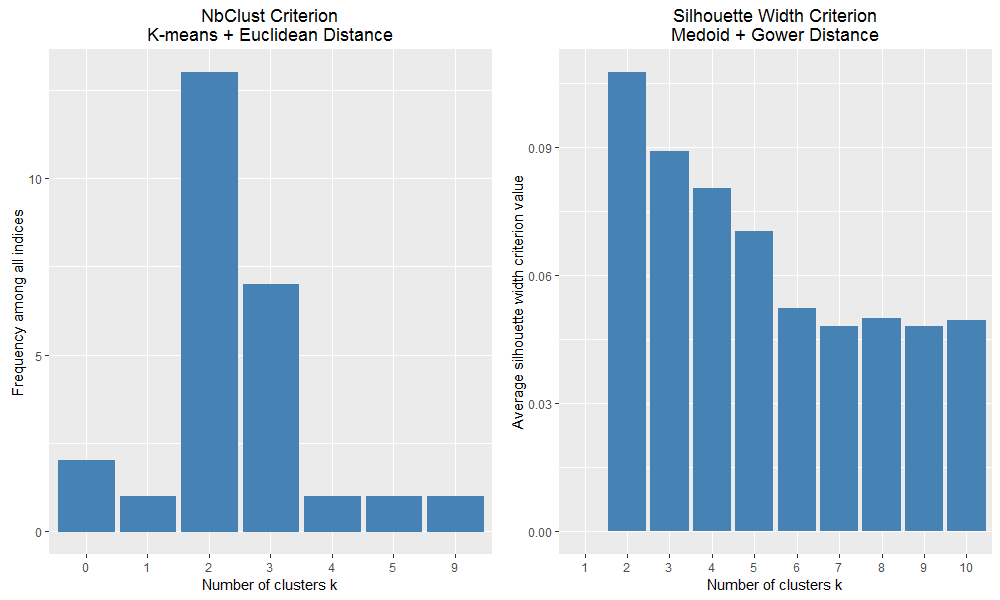
\includegraphics[width=5.20833in]{images/nonhier_kcrit.png}

We can see that the use of two clusters is reported to be optimal for
both clustering methods, while the use of three clusters is reported to
be the next best option.

With the number of clusters pre-determined based on these criteria, we
are able to move on to employing each non-hierarchical clustering
method. Below we show scatter plots which highlight the non-hierarchical
cluster assignments based on a two-dimensional reduction of our original
set of attitudinal survey responses.

\paragraph{Figure 3.4.2 Non-hierarchical Cluster
Plots}\label{figure-3.4.2-non-hierarchical-cluster-plots}

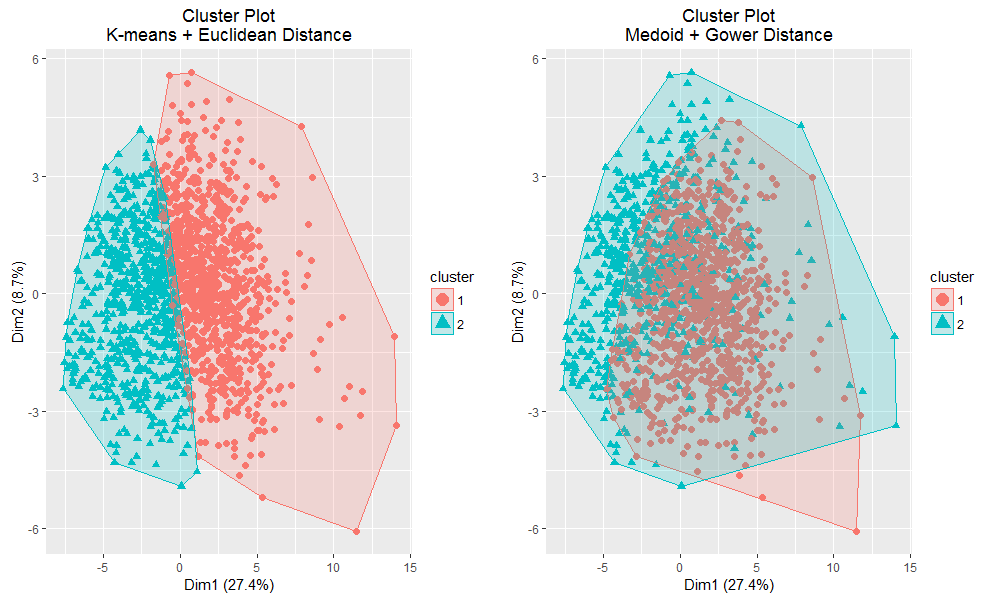
\includegraphics[width=5.20833in]{images/nonhier_clust.png}

In the above plots, the cluster boundaries are determined by connecting
the most extreme data points for each cluster. Interestingly, the medoid
cluster technique is shown to have a much greater overlap of clusters
than the k-means technique. Clearly, the overlap of cluster points and
therefore the inability to distinguish clusters can be seen as a
disadvantage for the Medoid cluster technique.

\subsubsection{3.5 Hierarchical
Clustering}\label{hierarchical-clustering}

For the hierarchical clustering method, we follow a similar process as
above to first determine an appropriate number of clusters. Although we
will assess all possible cluster options as part of a review of each
dendogram, a pre-determined number of clusters will aid in
interpretation of these plots. Again, we apply the `NbClust' function to
the ward clustering technique using both the Euclidean and Gower
distance metric.

\paragraph{Figure 3.5.1 Hierarchical Cluster
Criterion}\label{figure-3.5.1-hierarchical-cluster-criterion}

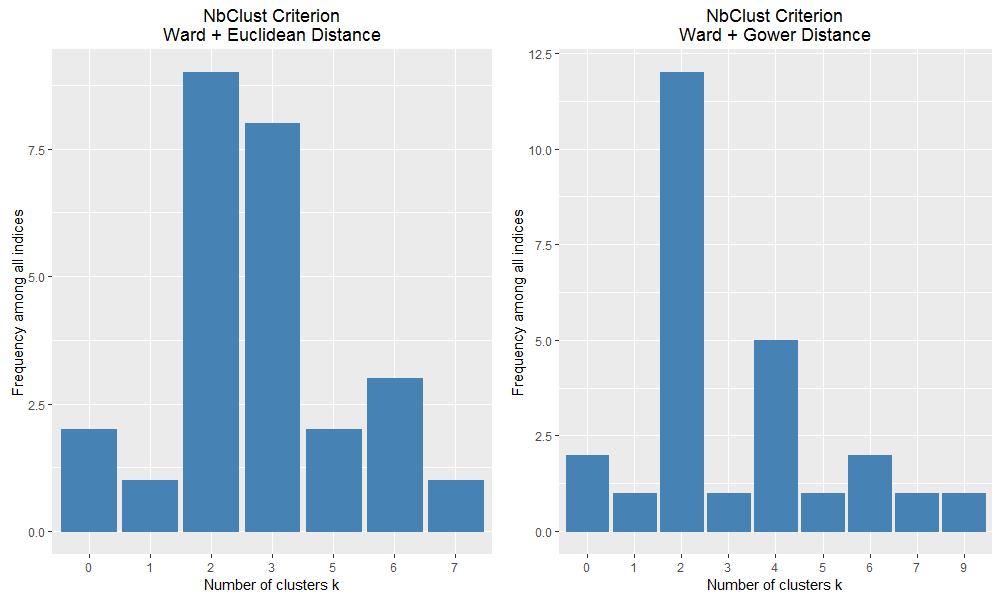
\includegraphics[width=5.20833in]{images/hier_kcrit.png}

We see that the use of three clusters is reported to be optimal when
using the Euclidean distance metric. When using the Gower distance
metric however, the use of two clusters is reported to be optimal. As
mentioned previously, hierarchical clustering methods are also able to
provide a dendogram to help assist in determining the number of
clusters. Dendograms for both distance metrics are shown below, colored
according to the use of their optimal number of clusters as reported by
the NbClust criterion.

\paragraph{Figure 3.5.2 Hierarchical Cluster
Dendogram}\label{figure-3.5.2-hierarchical-cluster-dendogram}

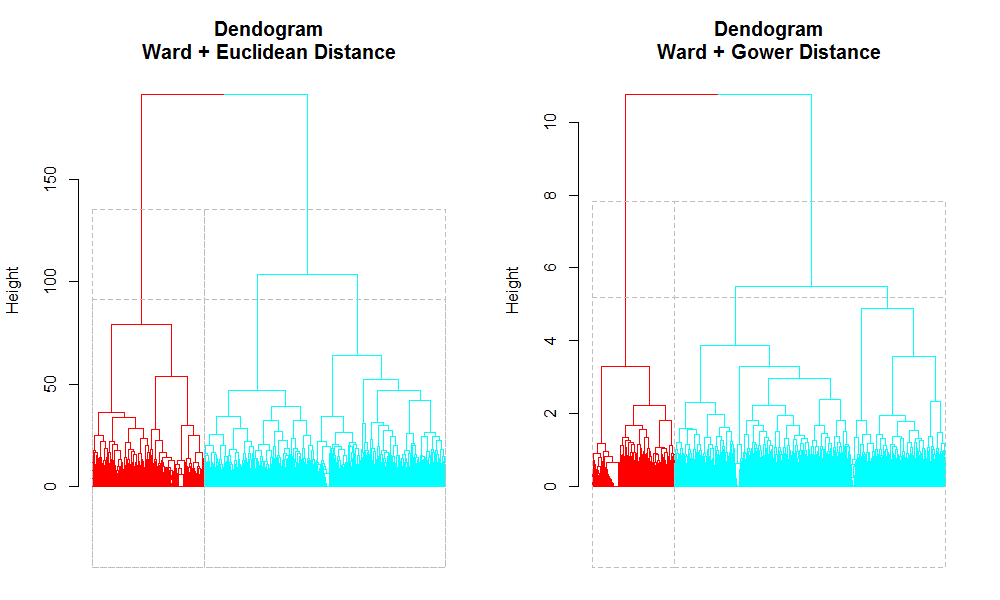
\includegraphics[width=5.20833in]{images/hier_den.png}

Determining the optimum `cut' using a dendogram is a subjective process.
Although there are some rules of thumb available (i.e.~clustering from
the top-down/bottom-up to include a minimum amount of leaves, or
excluding any early made branches with a minimum amount of leaves), the
practice is still likely to result in widely varying results between
analysts. For the two dendograms shown above, we have made the
assessment of three clusters being appropriate under both distance
metrics. We base this on an assessment of the amount of data points
included within each cluster. That is, making a cut after the second
Clade when using either distance metric, results in data points being
attributed fairly evenly between three clusters. Note that while the
NbClust criterion reported three clusters to be optimum when using the
Euclidean distance metric, however, four clusters was reported to be
inferior when using the Gower distance metric.

Below we show scatter plots which highlight the hierarchical cluster
assignments based on a two-dimensional reduction of our original set of
attitudinal survey responses.

\paragraph{Figure 3.5.3 Hierarchical Cluster
Plots}\label{figure-3.5.3-hierarchical-cluster-plots}

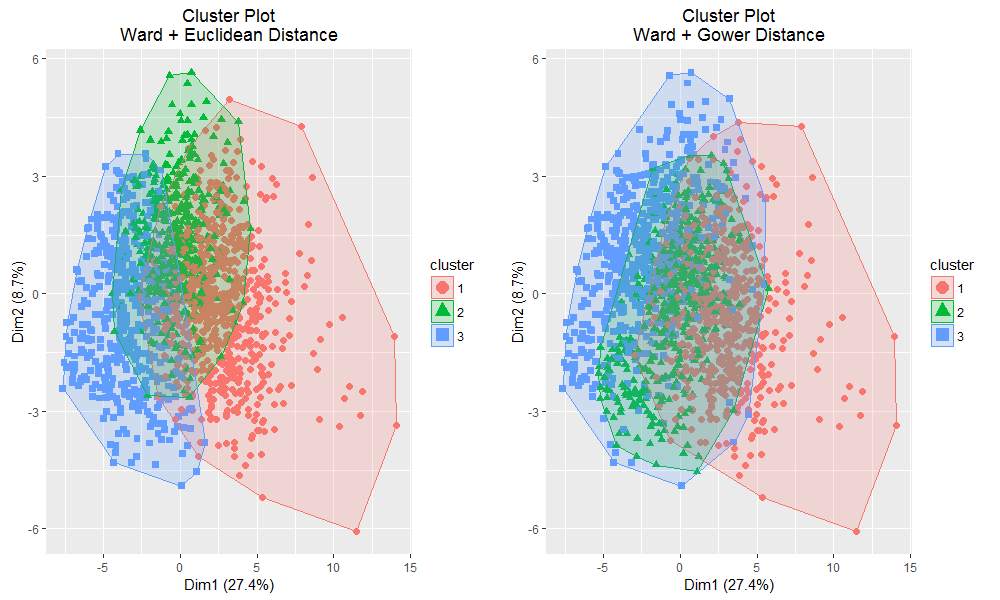
\includegraphics[width=5.20833in]{images/hier_clust.png}

Both are shown to have a large amount of overlap between clusters. In
particular, assigning three clusters according to the Euclidean distance
metric makes it difficult to distinguish the second cluster from the
remaining two clusters. And assigning three clusters according to the
Gower distance metric makes it difficult to distinguish the first and
third cluster.

\subsubsection{3.6 Statistical
Confirmation}\label{statistical-confirmation}

As a final evaluation of the performance of each clustering method, we
applied a generalized linear model to each question based on each
clustering method, and measured the models Akaike Information Criterion
(AIC) for each. We expect that generally, the lower the AIC value, the
more superior that clustering method is in predicting each cluster.

An assessment of the AIC value for each question reveals that each
clustering method tends to demonstrate low AIC values for questions two
and four, as well as high AIC values for questions one, and 56. This is
interesting as questions two and four are focused on the purchase
behavior of consumer segments, while questions one and 56 are focused on
characterizing the demographic features of each consumer segment.

We are also able to observe the average AIC value for each clustering
method in order to understand if a particular method is shown to have
superior predictive performance. A summary of the results for each is
shown in the table below.

\newpage

\paragraph{Table 3.6.1: AIC Comparison
Summary}\label{table-3.6.1-aic-comparison-summary}

\begin{longtable}[]{@{}lllll@{}}
\toprule
& 1 & 2 & 3 & 4\tabularnewline
\midrule
\endhead
Method & Non-Hierarchical & Non-Hierarchical & Hierarchical &
Hierarchical\tabularnewline
Technique & k-means & Medoid & Ward & Ward\tabularnewline
Distance Metric & Euclidean & Gower & Eucildean & Gower\tabularnewline
Number of Clusters & 2 & 2 & 3 & 3\tabularnewline
Mean AIC & 4025.706 & 4131.336 & 4015.816 & 4063.146\tabularnewline
\bottomrule
\end{longtable}

We can see that the Ward clustering technique with Eucildean distance
metric reported the lowest average AIC value, with the k-means
clustering technique with Eucildean distance metric reporting the second
lowest.

\subsubsection{3.7 Optimal Clustering
Method}\label{optimal-clustering-method}

Based on an assessment of the four combinations of clustering methods
and distance metric, we find the k-means clustering technique with
Euclidean distance to be the most favorable. This is largely based on
the technique's ability to distinguish between clusters with minimal
overlap over our two-dimensional data representations. We believe that
this technique's superior ability to distinguish between clusters should
ultimately improve our ability to draw inferences between clusters based
on their attitudinal characteristics. We do note the potential
shortcoming in leveraging a technique with the Euclidean distance
metric, namely that we are to assume the original dataset is of
continuous type. However, we feel that the encouraging results and
simplicity of this technique is well suited for the scope of this
analysis.

\subsection{4 Segment Profiling}\label{segment-profiling}

We employ visual methods in order to evaluate both the demographic and
consumer behavior characteristics of the two clusters determined by our
selected clustering method. We do this by generating a set of bar plots
of the total response count and proportion of responses over each
available option, for each question.

\subsubsection{4.1 Demographic
Characteristics}\label{demographic-characteristics}

We found a number of similarities over demographic characteristics for
both clusters. A similar proportion of respondents from both clusters
were either currently married, had no children, or were as likely to be
male or female. There were also similarities over the total number of
respondents for each cluster. We found for both clusters, there were
significantly more respondents who were younger than 35, college
graduates, white, married, had no children, and had a household annual
income of \$30,000 to \$70,000.

Fortunately, clusters were also able to be distinguished by a number of
demographic characteristics. The first cluster for example, was found to
contain a greater amount of younger respondents, who were more educated,
were more often white or Caucasian, or had higher incomes. To a lessor
extent, we also found this cluster to be more likely to have been
previously married but now separated, or to have older children than
those respondents from cluster two who also had children.

A number of plots related to the demographic characteristics for each
cluster can be found in Appendix A.

\subsubsection{4.2 Consumer Preferences}\label{consumer-preferences}

We again noted a number of similarities over consumer preferences for
both clusters. The majority of respondents owned an iPhone device, used
gaming or social networking applications, had in excess of 10
applications on their chosen device, or acquired at least half of their
device applications freely.

In terms of the differences in consumer preferences between clusters, we
found that respondents from the first cluster had a greater preference
for iPhone and Android devices and less of a preference for iPods and
tablet devices. In addition, the first cluster had less of a preference
for entertainment or T.V. applications, but a greater bias towards
gaming, music and social applications. Finally, respondents from the
first cluster were also found to have less applications, more free
applications and less likely to visit the websites designated by the
survey.

A number of plots related to the consumer preferences for each cluster
can be found in Appendix A.

\subsubsection{4.3 Initial Recommendation}\label{initial-recommendation}

Results from segment profiling indicate that the consumers within the
first cluster tend to have less of a preference for entertainment and
T.V. applications whilst more of a preference for social media
applications. Since AppHappy aim to produce a social entertainment
application, the results suggest that the social media aspect of the
product may have greater appeal to the first cluster, whilst the
entertainment aspect of the product may have greater appeal to the
second cluster.

The results indicated that consumers within the first cluster have a
preference for using iPhone and Android devices. If AppHappy were to
target a product at consumers designated by the first cluster, that
product would likely have greater adoption if it were made available on
these devices. The results also indicated that consumers within the
second cluster have a preference for using iPod and tablet devices, as
well as a greater tendency to browse those websites designated by the
survey (e.g.~Facebook and Twitter). If AppHappy were to target a product
at consumers designated by the second cluster, that product would likely
have greater adoption if it were made available on these devices and
advertised on websites designated by the survey.

\subsection{5 Predictive Classifier}\label{predictive-classifier}

AppHappy has requested that the segmentation results be used to inform a
classification model, which can ultimately be applied to future survey
data in order to generate meaningful customer segmentations. Such
classification models are able to derive predictors from observations
that are known, and apply those derived predictors to new observations
(E. Feit 2015).

There are many classification models which AppHappy could employ to
predict customer membership, with each model generally being categorized
according to their underlying algorithm. Three possible algorithms
include those based on a Decision Tree (DT), Support Vector Machine
(SVM), or K-Nearest Neighbors (KNN) methodology. A summary of the
strengths and weaknesses of each are shown below.

\subsubsection{5.1 Decision Tree}\label{decision-tree}

According to scikit learn, Decision Trees (DTs) are a non-parametric
supervised learning method used for classification and regression
(Scikit-Learn 2014). The goal is to create a model that predicts the
value of a target variable by learning simple decision rules inferred
from the data features.

Strengths:

\begin{itemize}
\tightlist
\item
  Fast training and testing phases.
\item
  Low memory usage.
\item
  Simple to understand and interpret.
\item
  Implicitly performs variable screening or feature selection.
\end{itemize}

Weaknesses:

\begin{itemize}
\tightlist
\item
  Has the tendency to overfit data.
\end{itemize}

\subsubsection{5.2 Support Vector Machine}\label{support-vector-machine}

According to scikit learn, Support Vector Machines (SVMs) are a set of
supervised learning methods used for classification, regression and
outliers detection (Scikit-Learn 2014). SVMs use a linear hyperplane in
order to separate data point, but can also be used as a non-linear
classified through the use of kernels.

Strengths:

\begin{itemize}
\tightlist
\item
  Low memory usage, as it only needs to store a subset of the data to
  make predictions.
\item
  SVM is effective in high dimensional spaces.
\item
  Versatile, as the kernel allows expert knowledge of the problem to be
  built into the classifier.
\end{itemize}

Weaknesses:

\begin{itemize}
\tightlist
\item
  Slow training and testing phases.
\end{itemize}

\subsubsection{5.3 K-Nearest Neighbors}\label{k-nearest-neighbors}

According to scikit learn, supervised neighbors-based learning methods
come in two flavors: classification for data with discrete labels, and
regression for data with continuous labels (Scikit-Learn 2014). The
principle behind nearest neighbor methods is to find a predefined number
of training samples closest in distance to the new point, and predict
the label from these.

Strengths:

\begin{itemize}
\tightlist
\item
  Fast training phase.
\item
  Versatile, as it does not make any assumption about the underlying
  data distribution.
\end{itemize}

Weaknesses:

\begin{itemize}
\tightlist
\item
  Slow testing phase.
\item
  High memory usage, as it requires storing all training data.
\end{itemize}

\subsubsection{5.4 Initial
Recommendation}\label{initial-recommendation-1}

It is difficult to recommend a classification model without directly
assessing the performance of each method. However, it is fair to say
that if the model is intended to be applied to large datasets where
CPU/memory constraints may be of issue, a DT or SVM based classifier may
be superior. On the other hand, if AppHappy intends on capturing data
which exhibits varying types, scale and distributions, than a KNeighbors
based classifier may be superior.

\subsection{6 Conclusion}\label{conclusion}

For this assessment, we applied a number combinations of clustering
techniques and distance metrics in order to segment survey data
according to three basis variables. Combinations involved the use of
hierarchical and non-hierarchical clustering methods under k-means,
medoid and ward techniques, as well as the use of Euclidean and Gower
distance metrics. While there were some noted concerns assuming the data
to be of continuous type, results showed the k-means clustering
technique with Euclidean distance metric to be the most favorable. This
was largely due to this methods ability to distinguish between clusters.

Respondents from both clusters were found to share many demographic and
behavioral characteristics, however a number of unique biases were also
identified. With respect to demographics, clusters were able to be
distinguished according to respondent age, ethnicity, education and
incomes. With respect to consumer attitudes, clusters were able to be
distinguished according to their preferences for type of electronic
device, use of applications and propensity to purchase rather than
freely download applications. Most notably, the first cluster was found
to have less of a preference for entertainment and T.V. applications,
more of a preference for social media applications, a greater preference
for using iPhone and Android devices, and less of a tendency to browse
those websites designated by the survey (e.g.~Facebook and Twitter).

There are many classification models which AppHappy could employ to
predict customer membership, with each model generally being categorized
according to their underlying algorithm. Three possible algorithms
include those based on a Decision Tree (DT), Support Vector Machine
(SVM), or K-Nearest Neighbors (KNN) methodology. This assessment
presented a summary of advantages and disadvantages associated with
each, however we note that a recommendation of classification model
would benefit from a direct assessment using the supplied data.

\newpage

\section{Appendix A Figure Output}\label{appendix-a-figure-output}

\subsubsection{Figure Set A1 Demographic
Characteristics}\label{figure-set-a1-demographic-characteristics}

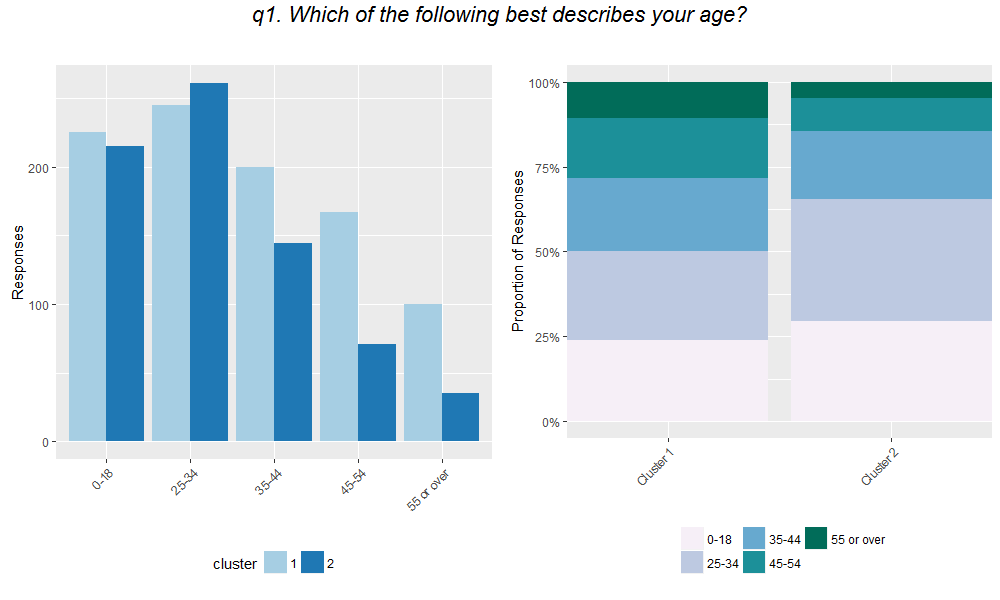
\includegraphics[width=6.25000in]{images/barplot_q1.recat.png}

~

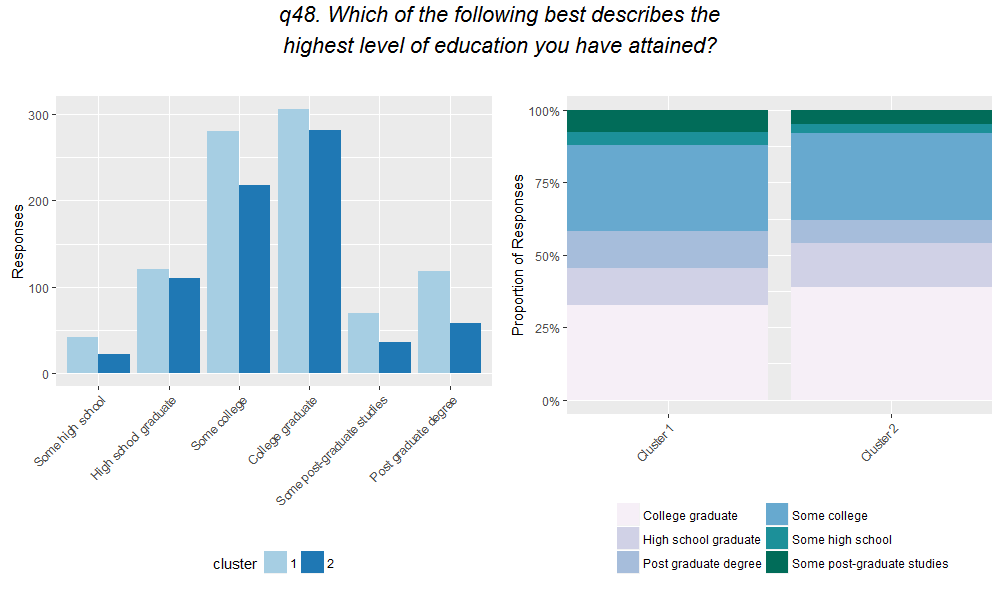
\includegraphics[width=6.25000in]{images/barplot_q48.png}

~

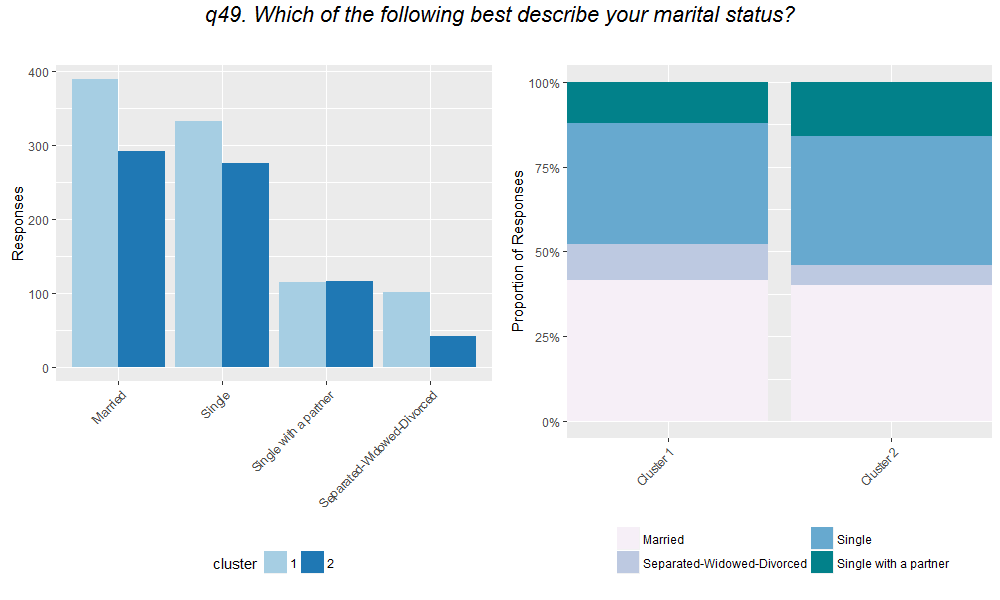
\includegraphics[width=6.25000in]{images/barplot_q49.png}

~

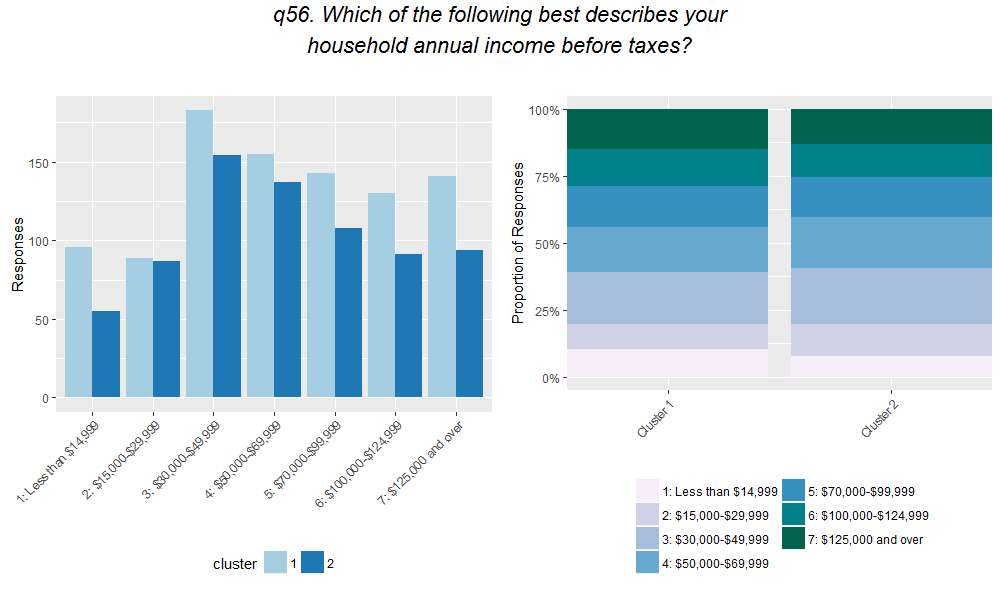
\includegraphics[width=6.25000in]{images/barplot_q56.recat.png}

\newpage

\subsubsection{Figure Set A2 Consumer
Preferences}\label{figure-set-a2-consumer-preferences}

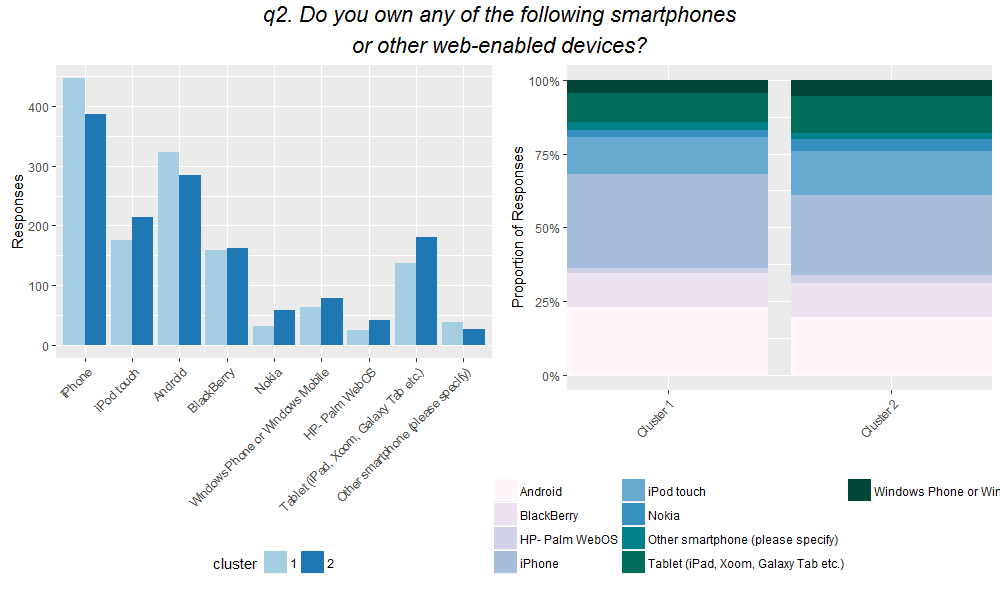
\includegraphics[width=6.25000in]{images/barplot_q2r1.png}

~

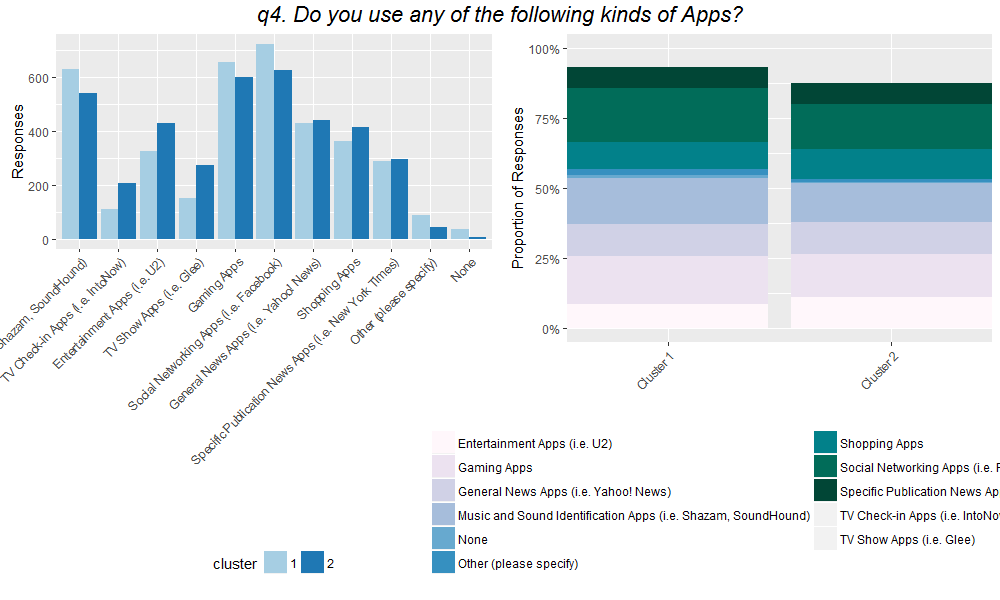
\includegraphics[width=6.25000in]{images/barplot_q4r1.png}

~

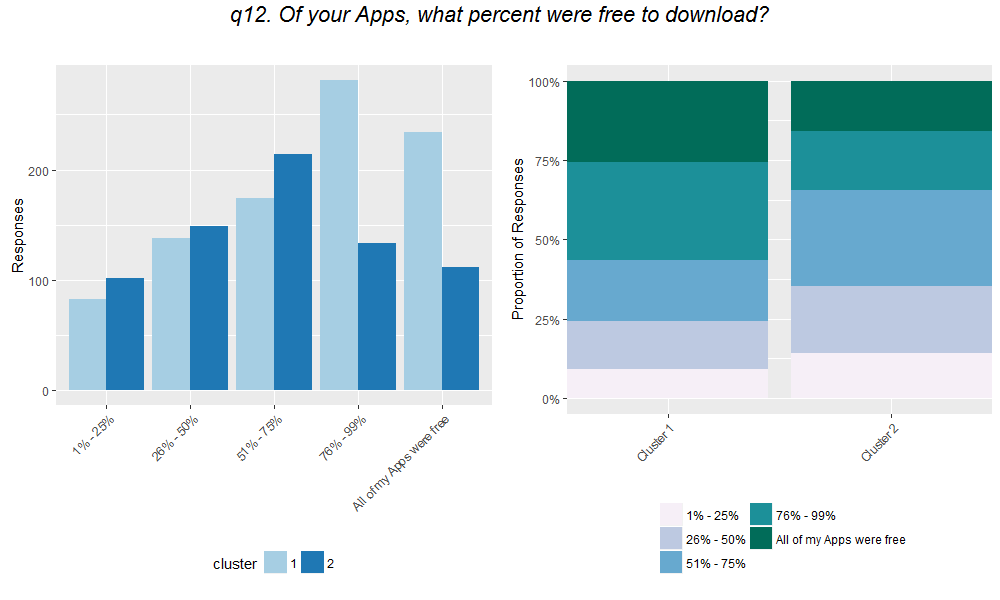
\includegraphics[width=6.25000in]{images/barplot_q12.recat.png}

~

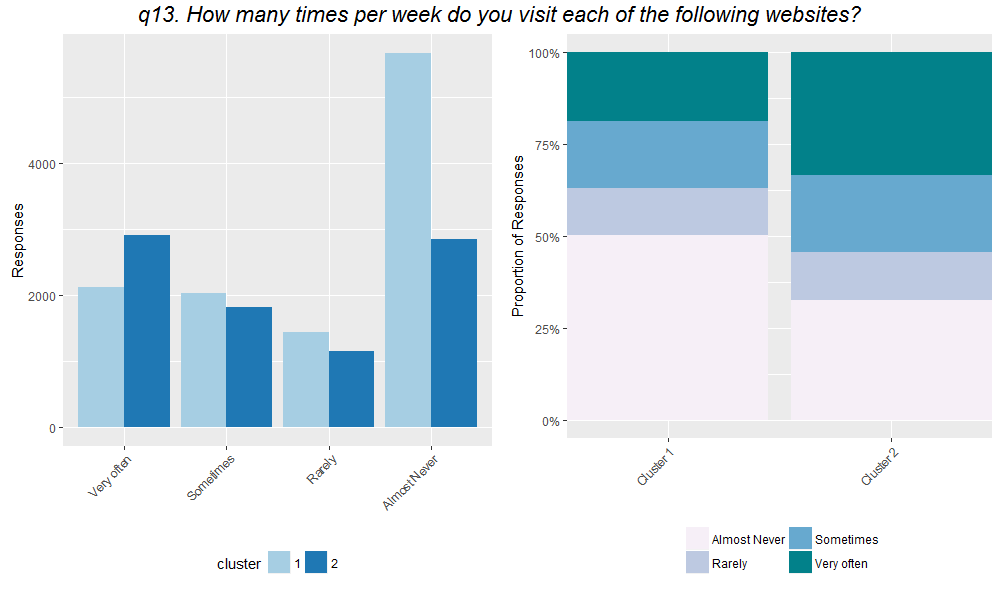
\includegraphics[width=6.25000in]{images/barplot_q13r1.png}

\newpage

\section{Appendix B Code}\label{appendix-b-code}

\subsubsection{B1 Data Prep}\label{b1-data-prep}

\begin{Shaded}
\begin{Highlighting}[]

\KeywordTok{for}\NormalTok{(package in c(}\StringTok{'cluster'}\NormalTok{, }\StringTok{'factoextra'}\NormalTok{, }\StringTok{'fpc'}\NormalTok{, }\StringTok{'NbClust'}\NormalTok{,}
                 \StringTok{'reshape'}\NormalTok{, }\StringTok{'plyr'}\NormalTok{,}
                 \StringTok{'ggplot2'}\NormalTok{, }\StringTok{'scales'}\NormalTok{, }\StringTok{'grid'}\NormalTok{, }\StringTok{'gridExtra'}\NormalTok{)) }\KeywordTok{\{}
  \KeywordTok{if}\NormalTok{(}\CommentTok{!require(package, character.only=TRUE)) \{}
    \NormalTok{install.packages(package)}
    \NormalTok{library(package, }\DataTypeTok{character}\NormalTok{.}\KeywordTok{only=}\NormalTok{TRUE)}
  \KeywordTok{\}}
\KeywordTok{\}}

\NormalTok{rm(package)}

\OtherTok{# Load the dataset}
\NormalTok{load(}\StringTok{'data/appHappyData-sp2016.RData'}\NormalTok{)}
\NormalTok{df_appnum.raw }\KeywordTok{<-} \NormalTok{apphappy}\FloatTok{.4}\KeywordTok{.num.}\NormalTok{frame}
\NormalTok{df_applab.raw }\KeywordTok{<-} \NormalTok{apphappy}\FloatTok{.4}\KeywordTok{.labs.}\NormalTok{frame}

\OtherTok{# Subset the data for attitudinal variables}
\CommentTok{colstart <- which(colnames(df_appnum.raw) == 'q24r1')}
\CommentTok{colend <- which(colnames(df_appnum.raw) == 'q26r17')}
\NormalTok{df_appnum.att }\KeywordTok{=} \NormalTok{df_appnum.raw}\KeywordTok{[}\NormalTok{,c(colstart:colend)}\KeywordTok{]}
\NormalTok{df_applab.att }\KeywordTok{=} \NormalTok{df_applab.raw}\KeywordTok{[}\NormalTok{,c(colstart:colend)}\KeywordTok{]}

\OtherTok{# Subset the data for nonattitudinal variables}
\NormalTok{df_appnum.nonatt }\KeywordTok{=} \NormalTok{df_appnum.raw}\KeywordTok{[}\NormalTok{,c(}\KeywordTok{-}\NormalTok{colstart:}\KeywordTok{-}\NormalTok{colend)}\KeywordTok{]}
\NormalTok{df_applab.nonatt }\KeywordTok{=} \NormalTok{df_applab.raw}\KeywordTok{[}\NormalTok{,c(}\KeywordTok{-}\NormalTok{colstart:}\KeywordTok{-}\NormalTok{colend)}\KeywordTok{]}

\OtherTok{# Count NA rows for attitudinal variables}
\NormalTok{inclna }\KeywordTok{<-} \NormalTok{nrow(df_appnum.att) }
\NormalTok{exclna }\KeywordTok{<-} \NormalTok{nrow(na.omit(df_appnum.att))}
\OtherTok{#print(paste0("Basis observations: ", inclna - exclna)) #0}

\OtherTok{# Count NA rows for non-attitudinal variables}
\NormalTok{inclna }\KeywordTok{<-} \NormalTok{nrow(df_appnum.nonatt) }
\NormalTok{exclna }\KeywordTok{<-} \NormalTok{nrow(na.omit(df_appnum.nonatt))}
\OtherTok{#print(paste0("Non-basis observations: ", inclna - exclna)) #585}

\OtherTok{# Count NA rows for original dataset}
\NormalTok{inclna }\KeywordTok{<-} \NormalTok{nrow(df_appnum.raw) }
\NormalTok{exclna }\KeywordTok{<-} \NormalTok{nrow(na.omit(df_appnum.raw))}
\OtherTok{#print(paste0("Dataset observations: ", inclna - exclna)) #585}

\NormalTok{rm(apphappy}\FloatTok{.4}\KeywordTok{.num.}\NormalTok{frame, apphappy}\FloatTok{.4}\KeywordTok{.labs.}\NormalTok{frame, colstart, colend)}
\end{Highlighting}
\end{Shaded}

\subsubsection{B2 Non-hierarchical
Clustering}\label{b2-non-hierarchical-clustering}

\begin{Shaded}
\begin{Highlighting}[]

\OtherTok{# Method: kmeans, Distance: euclidean}
\NormalTok{nbc.eu }\KeywordTok{<-} \NormalTok{NbClust(df_appnum.att, }
                  \KeywordTok{min}\NormalTok{.nc}\KeywordTok{=}\DecValTok{2}\NormalTok{, }\KeywordTok{max}\NormalTok{.nc}\KeywordTok{=}\DecValTok{10}\NormalTok{, distance}\KeywordTok{=}\StringTok{'euclidean'}\NormalTok{, }
                  \NormalTok{method}\KeywordTok{=}\StringTok{'kmeans'}\NormalTok{, }\KeywordTok{index=}\StringTok{'all'}\NormalTok{)}
\NormalTok{table(nc$Best.n}\KeywordTok{[}\DecValTok{1}\NormalTok{,}\KeywordTok{]}\NormalTok{)}

\NormalTok{plot1 }\KeywordTok{<-} \NormalTok{fviz_nbclust(nbc.eu) }\KeywordTok{+} 
  \NormalTok{ggtitle(}\StringTok{'NbClust Criterion\textbackslash{}nK-means + Euclidean Distance'}\NormalTok{)}

\NormalTok{rm(nbc.eu)}


\OtherTok{# Method: medoid, Distance: gower}
\NormalTok{dist.daisy }\KeywordTok{<-} \NormalTok{daisy(df_applab.att, metric}\KeywordTok{=}\StringTok{'gower'}\NormalTok{, stand}\KeywordTok{=}\NormalTok{FALSE)}
\NormalTok{pamk.gow }\KeywordTok{<-} \NormalTok{pamk(dist.daisy, diss}\KeywordTok{=}\NormalTok{TRUE, krange}\KeywordTok{=}\DecValTok{1}\NormalTok{:}\DecValTok{10}\NormalTok{, }
                 \NormalTok{criterion}\KeywordTok{=}\StringTok{'asw'}\NormalTok{, critout}\KeywordTok{=}\NormalTok{TRUE)}

\NormalTok{df_pamk }\KeywordTok{<-} \NormalTok{melt(pamk.gow$crit)}
\NormalTok{df_pamk$index }\KeywordTok{<-} \NormalTok{rownames(df_pamk)}

\NormalTok{plot3 }\KeywordTok{<-} \NormalTok{ggplot(df_pamk, aes(x}\KeywordTok{=index}\NormalTok{, y}\KeywordTok{=}\NormalTok{value)) }\KeywordTok{+}
  \NormalTok{geom_bar(stat}\KeywordTok{=}\StringTok{'identity'}\NormalTok{, fill}\KeywordTok{=}\StringTok{'steelblue'}\NormalTok{) }\KeywordTok{+} 
  \NormalTok{scale_x_discrete(limits}\KeywordTok{=}\NormalTok{c(}\DecValTok{1}\NormalTok{:}\DecValTok{10}\NormalTok{)) }\KeywordTok{+}
  \NormalTok{ggtitle(}\StringTok{'Silhouette Width Criterion\textbackslash{}nMedoid + Gower Distance'}\NormalTok{) }\KeywordTok{+}
  \NormalTok{labs(x}\KeywordTok{=}\StringTok{'Number of clusters k'}\NormalTok{, y}\KeywordTok{=}\StringTok{'Average silhouette width criterion value'}\NormalTok{)}

\NormalTok{rm(dist.daisy, pamk.gow, df_pamk)}


\NormalTok{png(filename}\KeywordTok{=}\StringTok{'images/nonhier_kcrit.png'}\NormalTok{, }
    \NormalTok{width }\KeywordTok{=} \DecValTok{1000}\NormalTok{, height }\KeywordTok{=} \DecValTok{600}\NormalTok{, res }\KeywordTok{=} \DecValTok{100}\NormalTok{)}

\NormalTok{grid.arrange(plot1, plot3, ncol}\KeywordTok{=}\DecValTok{2}\NormalTok{)}

\NormalTok{dev.off()}

\NormalTok{rm(plot1, plot2, plot3)}

\OtherTok{# Method: kmeans, Distance: euclidean}
\NormalTok{k }\KeywordTok{=} \DecValTok{2} \NormalTok{# Set cluster center }\FunctionTok{count} \NormalTok{according }\KeywordTok{to} \NormalTok{no. clust criterion}

\NormalTok{set.seed(}\DecValTok{1}\NormalTok{)}
\NormalTok{res.km }\KeywordTok{<-} \NormalTok{kmeans(df_appnum.att, centers}\KeywordTok{=}\NormalTok{k)}

\NormalTok{plot1 }\KeywordTok{<-} \NormalTok{fviz_cluster(res.km, df_appnum.att,}
                      \NormalTok{show}\KeywordTok{.clust.}\NormalTok{cent}\KeywordTok{=}\NormalTok{TRUE, geom}\KeywordTok{=}\StringTok{'point'}\NormalTok{,}
                      \NormalTok{title}\KeywordTok{=}\StringTok{'Cluster Plot\textbackslash{}nK-means + Euclidean Distance'}\NormalTok{)}


\OtherTok{# Method: medoid, Distance: gower}
\NormalTok{k }\KeywordTok{=} \DecValTok{2} \NormalTok{# Set cluster center }\FunctionTok{count} \NormalTok{according }\KeywordTok{to} \NormalTok{no. clust criterion}

\NormalTok{set.seed(}\DecValTok{1}\NormalTok{)}
\NormalTok{dist.daisy }\KeywordTok{<-} \NormalTok{daisy(df_applab.att, metric}\KeywordTok{=}\StringTok{'gower'}\NormalTok{, stand}\KeywordTok{=}\NormalTok{FALSE)}
\NormalTok{res.pam2 }\KeywordTok{<-} \NormalTok{pam(dist.daisy, k}\KeywordTok{=}\NormalTok{k, diss}\KeywordTok{=}\NormalTok{TRUE,}
                \NormalTok{metric}\KeywordTok{=}\StringTok{'euclidean'}\NormalTok{,}
                \NormalTok{stand}\KeywordTok{=}\NormalTok{FALSE, cluster.}\KeywordTok{only=}\NormalTok{FALSE)}

\NormalTok{plot3 }\KeywordTok{<-} \NormalTok{fviz_cluster(list(data}\KeywordTok{=}\NormalTok{df_appnum.att, }
                           \NormalTok{cluster}\KeywordTok{=}\NormalTok{res.pam2$cluster),}
                      \NormalTok{show}\KeywordTok{.clust.}\NormalTok{cent}\KeywordTok{=}\NormalTok{TRUE, geom}\KeywordTok{=}\StringTok{'point'}\NormalTok{,}
                      \NormalTok{title}\KeywordTok{=}\StringTok{'Cluster Plot\textbackslash{}nMedoid + Gower Distance'}\NormalTok{)}

\NormalTok{rm(dist.daisy)}


\NormalTok{png(filename}\KeywordTok{=}\StringTok{'images/nonhier_clust.png'}\NormalTok{, }
    \NormalTok{width }\KeywordTok{=} \DecValTok{1000}\NormalTok{, height }\KeywordTok{=} \DecValTok{600}\NormalTok{, res }\KeywordTok{=} \DecValTok{100}\NormalTok{)}

\NormalTok{grid.arrange(plot1, plot3, ncol}\KeywordTok{=}\DecValTok{2}\NormalTok{)}

\NormalTok{dev.off()}

\NormalTok{rm(plot1, plot2, plot3)}
\NormalTok{rm(k)}
\end{Highlighting}
\end{Shaded}

\subsubsection{B3 Hierarchical
Clustering}\label{b3-hierarchical-clustering}

\begin{Shaded}
\begin{Highlighting}[]

\OtherTok{# Method: ward.D, Distance: euclidean}
\NormalTok{nbc.eu }\KeywordTok{<-} \NormalTok{NbClust(df_appnum.att, diss}\KeywordTok{=}\NormalTok{NULL,}
                  \KeywordTok{min}\NormalTok{.nc}\KeywordTok{=}\DecValTok{2}\NormalTok{, }\KeywordTok{max}\NormalTok{.nc}\KeywordTok{=}\DecValTok{10}\NormalTok{, distance}\KeywordTok{=}\StringTok{'euclidean'}\NormalTok{,}
                  \NormalTok{method}\KeywordTok{=}\StringTok{'ward.D2'}\NormalTok{, }\KeywordTok{index=}\StringTok{'all'}\NormalTok{)}
\NormalTok{table(nbc.eu$Best.n}\KeywordTok{[}\DecValTok{1}\NormalTok{,}\KeywordTok{]}\NormalTok{)}

\NormalTok{plot1 }\KeywordTok{<-} \NormalTok{fviz_nbclust(nbc.eu) }\KeywordTok{+} 
  \NormalTok{ggtitle(}\StringTok{'NbClust Criterion\textbackslash{}nWard + Euclidean Distance'}\NormalTok{)}


\OtherTok{# Method: ward.D, Distance: manhattan}
\NormalTok{nbc.man }\KeywordTok{<-} \NormalTok{NbClust(df_appnum.att, diss}\KeywordTok{=}\NormalTok{NULL,}
                   \KeywordTok{min}\NormalTok{.nc}\KeywordTok{=}\DecValTok{2}\NormalTok{, }\KeywordTok{max}\NormalTok{.nc}\KeywordTok{=}\DecValTok{10}\NormalTok{, distance}\KeywordTok{=}\StringTok{'manhattan'}\NormalTok{,}
                   \NormalTok{method}\KeywordTok{=}\StringTok{'ward.D2'}\NormalTok{, }\KeywordTok{index=}\StringTok{'all'}\NormalTok{)}
\NormalTok{table(nbc.man$Best.n}\KeywordTok{[}\DecValTok{1}\NormalTok{,}\KeywordTok{]}\NormalTok{)}

\NormalTok{plot2 }\KeywordTok{<-} \NormalTok{fviz_nbclust(nbc.eu) }\KeywordTok{+} 
  \NormalTok{ggtitle(}\StringTok{'NbClust Criterion\textbackslash{}nWard + Manhattan Distance'}\NormalTok{)}


\OtherTok{# Method: ward.D, Distance: gower}
\NormalTok{dist.daisy }\KeywordTok{<-} \NormalTok{daisy(df_applab.att, metric}\KeywordTok{=}\StringTok{'gower'}\NormalTok{, stand}\KeywordTok{=}\NormalTok{FALSE)}
\NormalTok{nbc.gow }\KeywordTok{<-} \NormalTok{NbClust(df_appnum.att, diss}\KeywordTok{=}\NormalTok{dist.daisy,}
                   \KeywordTok{min}\NormalTok{.nc}\KeywordTok{=}\DecValTok{2}\NormalTok{, }\KeywordTok{max}\NormalTok{.nc}\KeywordTok{=}\DecValTok{10}\NormalTok{, distance}\KeywordTok{=}\NormalTok{NULL,}
                   \NormalTok{method}\KeywordTok{=}\StringTok{'ward.D2'}\NormalTok{, }\KeywordTok{index=}\StringTok{'all'}\NormalTok{)}
\NormalTok{table(nbc.gow$Best.n}\KeywordTok{[}\DecValTok{1}\NormalTok{,}\KeywordTok{]}\NormalTok{)}

\NormalTok{plot3 }\KeywordTok{<-} \NormalTok{fviz_nbclust(nbc.gow) }\KeywordTok{+} 
  \NormalTok{ggtitle(}\StringTok{'NbClust Criterion\textbackslash{}nWard + Gower Distance'}\NormalTok{)}


\NormalTok{png(filename}\KeywordTok{=}\StringTok{'images/hier_kcrit.png'}\NormalTok{, }
    \NormalTok{width }\KeywordTok{=} \DecValTok{1000}\NormalTok{, height }\KeywordTok{=} \DecValTok{600}\NormalTok{, res }\KeywordTok{=} \DecValTok{100}\NormalTok{)}

\NormalTok{grid.arrange(plot1, plot3, ncol}\KeywordTok{=}\DecValTok{2}\NormalTok{)}

\NormalTok{dev.off()}

\NormalTok{rm(plot1, plot2, plot3)}

\OtherTok{# Method: ward.D, Distance: euclidean}
\NormalTok{k }\KeywordTok{=} \DecValTok{3} \NormalTok{# Color dendogram according }\KeywordTok{to} \NormalTok{no. clust criterion}

\NormalTok{set.seed(}\DecValTok{1}\NormalTok{)}
\NormalTok{res.hcut1 }\KeywordTok{<-} \NormalTok{hcut(df_appnum.att, k}\KeywordTok{=}\NormalTok{k, isdiss}\KeywordTok{=}\NormalTok{FALSE, }
                  \NormalTok{hc_func}\KeywordTok{=}\StringTok{'hclust'}\NormalTok{, hc_metric}\KeywordTok{=}\StringTok{'euclidean'}\NormalTok{,}
                  \NormalTok{hc_method}\KeywordTok{=}\StringTok{'ward.D2'}\NormalTok{, stand}\KeywordTok{=}\NormalTok{FALSE)}

\NormalTok{plot1a }\KeywordTok{<-} \NormalTok{fviz_silhouette(res.hcut1) }\KeywordTok{+}
  \NormalTok{scale_y_continuous(limits }\KeywordTok{=} \NormalTok{c(}\KeywordTok{-}\FloatTok{0.25}\NormalTok{, }\FloatTok{0.5}\NormalTok{)) }\KeywordTok{+}
  \NormalTok{ggtitle(}\StringTok{'Silhouette Plot\textbackslash{}nWard + Euclidean Distance'}\NormalTok{) }\KeywordTok{+}
  \NormalTok{theme(axis}\KeywordTok{.text.}\NormalTok{x }\KeywordTok{=} \NormalTok{element_blank(), axis}\KeywordTok{.ticks.}\NormalTok{x }\KeywordTok{=} \NormalTok{element_blank())}

\NormalTok{plot1b }\KeywordTok{<-} \NormalTok{fviz_cluster(res.hcut1, df_appnum.att, }
                      \NormalTok{show}\KeywordTok{.clust.}\NormalTok{cent}\KeywordTok{=}\NormalTok{TRUE, geom}\KeywordTok{=}\StringTok{'point'}\NormalTok{,}
                      \NormalTok{title}\KeywordTok{=}\StringTok{'Cluster Plot\textbackslash{}nWard + Euclidean Distance'}\NormalTok{)}


\OtherTok{# Method: ward.D, Distance: gower}
\NormalTok{k }\KeywordTok{=} \DecValTok{2} \NormalTok{# Color dendogram according }\KeywordTok{to} \NormalTok{no. clust criterion}

\NormalTok{set.seed(}\DecValTok{1}\NormalTok{)}
\NormalTok{dist.daisy }\KeywordTok{<-} \NormalTok{daisy(df_applab.att, metric}\KeywordTok{=}\StringTok{'gower'}\NormalTok{, stand}\KeywordTok{=}\NormalTok{FALSE)}
\NormalTok{res.hcut3 }\KeywordTok{<-} \NormalTok{hcut(dist.daisy, k}\KeywordTok{=}\NormalTok{k, isdiss}\KeywordTok{=}\NormalTok{TRUE,}
                  \NormalTok{hc_func}\KeywordTok{=}\StringTok{'hclust'}\NormalTok{, hc_metric}\KeywordTok{=}\StringTok{'euclidean'}\NormalTok{,}
                  \NormalTok{hc_method}\KeywordTok{=}\StringTok{'ward.D2'}\NormalTok{, stand}\KeywordTok{=}\NormalTok{FALSE)}

\NormalTok{plot3a }\KeywordTok{<-} \NormalTok{fviz_silhouette(res.hcut3) }\KeywordTok{+}
  \NormalTok{scale_y_continuous(limits }\KeywordTok{=} \NormalTok{c(}\KeywordTok{-}\FloatTok{0.25}\NormalTok{, }\FloatTok{0.5}\NormalTok{)) }\KeywordTok{+}
  \NormalTok{ggtitle(}\StringTok{'Silhouette Plot\textbackslash{}nWard + Gower Distance'}\NormalTok{) }\KeywordTok{+}
  \NormalTok{theme(axis}\KeywordTok{.text.}\NormalTok{x }\KeywordTok{=} \NormalTok{element_blank(), axis}\KeywordTok{.ticks.}\NormalTok{x }\KeywordTok{=} \NormalTok{element_blank())}

\NormalTok{plot3b }\KeywordTok{<-} \NormalTok{fviz_cluster(res.hcut3, df_appnum.att, }
                      \NormalTok{show}\KeywordTok{.clust.}\NormalTok{cent}\KeywordTok{=}\NormalTok{TRUE, geom}\KeywordTok{=}\StringTok{'point'}\NormalTok{,}
                      \NormalTok{title}\KeywordTok{=}\StringTok{'Cluster Plot\textbackslash{}nWard + Gower Distance'}\NormalTok{)}

\NormalTok{rm(dist.daisy)}


\NormalTok{png(filename}\KeywordTok{=}\StringTok{'images/hier_den.png'}\NormalTok{, }
    \NormalTok{width }\KeywordTok{=} \DecValTok{1000}\NormalTok{, height }\KeywordTok{=} \DecValTok{600}\NormalTok{, res }\KeywordTok{=} \DecValTok{100}\NormalTok{)}

\NormalTok{par(mfrow}\KeywordTok{=}\NormalTok{c(}\DecValTok{1}\NormalTok{,}\DecValTok{2}\NormalTok{))}

\NormalTok{fviz_dend(res.hcut1, k}\KeywordTok{=}\DecValTok{3}\NormalTok{, }
          \NormalTok{cex}\KeywordTok{=}\FloatTok{0.5}\NormalTok{, show_labels}\KeywordTok{=}\NormalTok{FALSE, rect}\KeywordTok{=}\NormalTok{TRUE,}
          \NormalTok{main}\KeywordTok{=}\StringTok{'Dendogram\textbackslash{}nWard + Euclidean Distance'}\NormalTok{)}

\NormalTok{fviz_dend(res.hcut3, k}\KeywordTok{=}\DecValTok{2}\NormalTok{,}
          \NormalTok{cex}\KeywordTok{=}\FloatTok{0.5}\NormalTok{, show_labels}\KeywordTok{=}\NormalTok{FALSE, rect}\KeywordTok{=}\NormalTok{TRUE,}
          \NormalTok{main}\KeywordTok{=}\StringTok{'Dendogram\textbackslash{}nWard + Gower Distance'}\NormalTok{)}

\NormalTok{par()}
\NormalTok{dev.off()}


\OtherTok{# Method: ward.D, Distance: gower}
\NormalTok{k }\KeywordTok{=} \DecValTok{3} \NormalTok{# Re}\KeywordTok{-}\NormalTok{run }\KeywordTok{for} \NormalTok{four clusters based on interpretation of dendogram}

\NormalTok{set.seed(}\DecValTok{1}\NormalTok{)}
\NormalTok{dist.daisy }\KeywordTok{<-} \NormalTok{daisy(df_applab.att, metric}\KeywordTok{=}\StringTok{'gower'}\NormalTok{, stand}\KeywordTok{=}\NormalTok{FALSE)}
\NormalTok{res.hcut3 }\KeywordTok{<-} \NormalTok{hcut(dist.daisy, k}\KeywordTok{=}\NormalTok{k, isdiss}\KeywordTok{=}\NormalTok{TRUE,}
                  \NormalTok{hc_func}\KeywordTok{=}\StringTok{'hclust'}\NormalTok{, hc_metric}\KeywordTok{=}\StringTok{'euclidean'}\NormalTok{,}
                  \NormalTok{hc_method}\KeywordTok{=}\StringTok{'ward.D2'}\NormalTok{, stand}\KeywordTok{=}\NormalTok{FALSE)}

\NormalTok{plot3a }\KeywordTok{<-} \NormalTok{fviz_silhouette(res.hcut3) }\KeywordTok{+}
  \NormalTok{scale_y_continuous(limits }\KeywordTok{=} \NormalTok{c(}\KeywordTok{-}\FloatTok{0.25}\NormalTok{, }\FloatTok{0.5}\NormalTok{)) }\KeywordTok{+}
  \NormalTok{ggtitle(}\StringTok{'Silhouette Plot\textbackslash{}nWard + Gower Distance'}\NormalTok{) }\KeywordTok{+}
  \NormalTok{theme(axis}\KeywordTok{.text.}\NormalTok{x }\KeywordTok{=} \NormalTok{element_blank(), axis}\KeywordTok{.ticks.}\NormalTok{x }\KeywordTok{=} \NormalTok{element_blank())}

\NormalTok{plot3b }\KeywordTok{<-} \NormalTok{fviz_cluster(res.hcut3, df_appnum.att, }
                       \NormalTok{show}\KeywordTok{.clust.}\NormalTok{cent}\KeywordTok{=}\NormalTok{TRUE, geom}\KeywordTok{=}\StringTok{'point'}\NormalTok{,}
                       \NormalTok{title}\KeywordTok{=}\StringTok{'Cluster Plot\textbackslash{}nWard + Gower Distance'}\NormalTok{)}

\NormalTok{rm(dist.daisy)}


\NormalTok{png(filename}\KeywordTok{=}\StringTok{'images/hier_sil.png'}\NormalTok{, }
    \NormalTok{width }\KeywordTok{=} \DecValTok{1000}\NormalTok{, height }\KeywordTok{=} \DecValTok{600}\NormalTok{, res }\KeywordTok{=} \DecValTok{100}\NormalTok{)}

\NormalTok{grid.arrange(plot1a, plot3a, ncol}\KeywordTok{=}\DecValTok{2}\NormalTok{)}

\NormalTok{dev.off()}

\NormalTok{rm(plot1a, plot2a, plot3a)}

\NormalTok{png(filename}\KeywordTok{=}\StringTok{'images/hier_clust.png'}\NormalTok{, }
    \NormalTok{width }\KeywordTok{=} \DecValTok{1000}\NormalTok{, height }\KeywordTok{=} \DecValTok{600}\NormalTok{, res }\KeywordTok{=} \DecValTok{100}\NormalTok{)}

\NormalTok{grid.arrange(plot1b, plot3b, ncol}\KeywordTok{=}\DecValTok{2}\NormalTok{)}

\NormalTok{dev.off()}

\NormalTok{rm(plot1b, plot2b, plot3b)}
\NormalTok{rm(k)}
\end{Highlighting}
\end{Shaded}

\subsubsection{B4 Statistical
Confirmation}\label{b4-statistical-confirmation}

\begin{Shaded}
\begin{Highlighting}[]

\NormalTok{ls_nm }\KeywordTok{<-} \NormalTok{list(}\StringTok{'res.km'}\NormalTok{, }\StringTok{'res.pam2'}\NormalTok{, }\StringTok{'res.hcut1'}\NormalTok{, }\StringTok{'res.hcut3'}\NormalTok{)}
\NormalTok{ls_df }\KeywordTok{<-} \NormalTok{list(res.km, res.pam2, res.hcut1, res.hcut3)}

\OtherTok{# Calculate the AIC for each clustering method, for each question}
\NormalTok{apply}\KeywordTok{.glm.}\NormalTok{f }\KeywordTok{<-} \KeywordTok{function}\NormalTok{(y,class)}\KeywordTok{\{}
  \KeywordTok{return}\NormalTok{(glm(y}\KeywordTok{~}\NormalTok{class)$aic)}
\KeywordTok{\}}

\NormalTok{df_temp }\KeywordTok{<-} \NormalTok{data.frame(names }\KeywordTok{=} \NormalTok{rownames(t(df_appnum.raw)))}

\KeywordTok{for} \NormalTok{(i in }\DecValTok{1}\NormalTok{:length(ls_nm))}\KeywordTok{\{}
  \NormalTok{df_appnum.raw$cluster }\KeywordTok{<-} \NormalTok{ls_df}\KeywordTok{[[}\NormalTok{i}\KeywordTok{]]}\NormalTok{$cluster}
  \NormalTok{df_aic }\KeywordTok{<-} \NormalTok{data.frame(apply(df_appnum.raw, }\DecValTok{2}\NormalTok{, }
                             \NormalTok{apply}\KeywordTok{.glm.}\NormalTok{f, class}\KeywordTok{=}\NormalTok{df_appnum.raw$cluster))}
  \NormalTok{names(df_aic)}\KeywordTok{[}\DecValTok{1}\KeywordTok{]} \KeywordTok{<-} \NormalTok{ls_nm}\KeywordTok{[[}\NormalTok{i}\KeywordTok{]]}
  \NormalTok{df_aic$names }\KeywordTok{<-} \NormalTok{rownames(df_aic)}
  
  \NormalTok{df_temp }\KeywordTok{<-} \KeywordTok{merge}\NormalTok{(x}\KeywordTok{=}\NormalTok{df_temp, y}\KeywordTok{=}\NormalTok{df_aic, by.x}\KeywordTok{=}\StringTok{'names'}\NormalTok{, }\FunctionTok{all}\KeywordTok{=}\NormalTok{TRUE)}
\KeywordTok{\}}

\NormalTok{rownames(df_temp) }\KeywordTok{<-} \NormalTok{df_temp}\KeywordTok{[}\NormalTok{, }\DecValTok{1}\KeywordTok{]}
\NormalTok{df_temp }\KeywordTok{<-} \NormalTok{df_temp}\KeywordTok{[-}\NormalTok{c(}\DecValTok{1}\NormalTok{:}\DecValTok{2}\NormalTok{),}\KeywordTok{-}\DecValTok{1}\KeywordTok{]}

\NormalTok{df_aic }\KeywordTok{<-} \NormalTok{df_temp}\KeywordTok{[}\NormalTok{is.finite(rowSums(df_temp)), }\KeywordTok{]}
\CommentTok{colnames(df_aic) <- c('k-means + Euclidean', 'Medoid + Gower',}
                      \StringTok{'Ward + Eucildean'}\NormalTok{, }\StringTok{'Ward + Gower'}\NormalTok{)}
\FunctionTok{write}\NormalTok{.table(round(df_aic, }\DecValTok{3}\NormalTok{), }\StringTok{'aic.csv'}\NormalTok{)}
\NormalTok{apply(df_aic, }\DecValTok{2}\NormalTok{, mean)}


\OtherTok{# Calculate the Chi for each clustering method, for each question}
\NormalTok{sim}\KeywordTok{.chisq.}\NormalTok{pval.f }\KeywordTok{<-} \KeywordTok{function}\NormalTok{(x,class)}\KeywordTok{\{}
  \KeywordTok{return}\NormalTok{(chisq.test(x,class,}
                    \NormalTok{rescale.p}\KeywordTok{=}\NormalTok{TRUE,}
                    \NormalTok{simulate}\KeywordTok{.p.}\NormalTok{value}\KeywordTok{=}\NormalTok{TRUE)$p.value)}
\KeywordTok{\}}

\NormalTok{df_temp }\KeywordTok{<-} \NormalTok{data.frame(names }\KeywordTok{=} \NormalTok{rownames(t(df_appnum.raw)))}

\KeywordTok{for} \NormalTok{(i in }\DecValTok{1}\NormalTok{:length(ls_nm))}\KeywordTok{\{}
  \NormalTok{df_appnum.raw$cluster }\KeywordTok{<-} \NormalTok{ls_df}\KeywordTok{[[}\NormalTok{i}\KeywordTok{]]}\NormalTok{$cluster}
  \NormalTok{df_chi }\KeywordTok{<-} \NormalTok{data.frame(apply(df_appnum.att, }\DecValTok{2}\NormalTok{,}
                             \NormalTok{sim}\KeywordTok{.chisq.}\NormalTok{pval.f, class}\KeywordTok{=}\NormalTok{df_appnum.raw$cluster))}
  \NormalTok{names(df_chi)}\KeywordTok{[}\DecValTok{1}\KeywordTok{]} \KeywordTok{<-} \NormalTok{ls_nm}\KeywordTok{[[}\NormalTok{i}\KeywordTok{]]}
  \NormalTok{df_chi$names }\KeywordTok{<-} \NormalTok{rownames(df_chi)}
  
  \NormalTok{df_temp }\KeywordTok{<-} \KeywordTok{merge}\NormalTok{(x}\KeywordTok{=}\NormalTok{df_temp, y}\KeywordTok{=}\NormalTok{df_chi, by.x}\KeywordTok{=}\StringTok{'names'}\NormalTok{, }\FunctionTok{all}\KeywordTok{=}\NormalTok{TRUE)}
\KeywordTok{\}}

\NormalTok{rownames(df_temp) }\KeywordTok{<-} \NormalTok{df_temp}\KeywordTok{[}\NormalTok{, }\DecValTok{1}\KeywordTok{]}
\NormalTok{df_temp }\KeywordTok{<-} \NormalTok{df_temp}\KeywordTok{[-}\NormalTok{c(}\DecValTok{1}\NormalTok{:}\DecValTok{2}\NormalTok{),}\KeywordTok{-}\DecValTok{1}\KeywordTok{]}

\NormalTok{df_chi }\KeywordTok{<-} \NormalTok{df_temp}\KeywordTok{[}\NormalTok{is.finite(rowSums(df_temp)), }\KeywordTok{]}
\CommentTok{colnames(df_chi) <- c('k-means + Euclidean', 'Medoid + Gower',}
                      \StringTok{'Ward + Eucildean'}\NormalTok{, }\StringTok{'Ward + Gower'}\NormalTok{)}
\NormalTok{apply(df_chi, }\DecValTok{2}\NormalTok{, mean)}


\NormalTok{rm(ls_nm, ls_df, df_temp)}
\end{Highlighting}
\end{Shaded}

\subsubsection{B5 Cluster Exploration}\label{b5-cluster-exploration}

\begin{Shaded}
\begin{Highlighting}[]

\OtherTok{# Select clustering method}
\NormalTok{res.sel }\KeywordTok{<-} \NormalTok{res.km # res.km, res.pam1, res.pam2, res.hcut1, res.hcut2, res.hcut3}
\NormalTok{df_appnum.raw$cluster }\KeywordTok{<-} \NormalTok{res.sel$cluster}
\NormalTok{df_applab.raw$cluster }\KeywordTok{<-} \NormalTok{res.sel$cluster}

\NormalTok{df_means }\KeywordTok{<-} \NormalTok{ddply(df_appnum.raw, }
                  \NormalTok{.(df_appnum.raw$cluster), colwise(mean))}

\OtherTok{# Basic Cluster Profiling}
\NormalTok{with(df_applab.raw, table(q1, cluster))}
\NormalTok{with(df_applab.raw, table(q11, cluster))}
\NormalTok{with(df_applab.raw, table(q12, cluster))}
\NormalTok{with(df_applab.raw, table(q48, cluster))}
\NormalTok{with(df_applab.raw, table(q49, cluster))}
\NormalTok{with(df_applab.raw, table(q54, cluster))}
\NormalTok{with(df_applab.raw, table(q56, cluster))}

\NormalTok{plot(df_means$q1, }\DataTypeTok{type}\KeywordTok{=}\StringTok{'b'}\NormalTok{, main}\KeywordTok{=}\StringTok{'Age by Cluster'}\NormalTok{)}
\NormalTok{plot(df_means$q11, }\DataTypeTok{type}\KeywordTok{=}\StringTok{'b'}\NormalTok{, main}\KeywordTok{=}\StringTok{'# of Apps by Cluster'}\NormalTok{)}
\NormalTok{plot(df_means$q12, }\DataTypeTok{type}\KeywordTok{=}\StringTok{'b'}\NormalTok{, main}\KeywordTok{=}\StringTok{'% of Free Apps by Cluster'}\NormalTok{)}
\NormalTok{plot(df_means$q48, }\DataTypeTok{type}\KeywordTok{=}\StringTok{'b'}\NormalTok{, main}\KeywordTok{=}\StringTok{'Education by Cluster'}\NormalTok{)}
\NormalTok{plot(df_means$q49, }\DataTypeTok{type}\KeywordTok{=}\StringTok{'b'}\NormalTok{, main}\KeywordTok{=}\StringTok{'Martial Status by Cluster'}\NormalTok{)}
\NormalTok{plot(df_means$q54, }\DataTypeTok{type}\KeywordTok{=}\StringTok{'b'}\NormalTok{, main}\KeywordTok{=}\StringTok{'Ethnicity by Cluster'}\NormalTok{)}
\NormalTok{plot(df_means$q56, }\DataTypeTok{type}\KeywordTok{=}\StringTok{'b'}\NormalTok{, main}\KeywordTok{=}\StringTok{'Income by Cluster'}\NormalTok{)}

\NormalTok{anova(aov(q1}\KeywordTok{~}\NormalTok{cluster, data}\KeywordTok{=}\NormalTok{df_appnum.raw))}
\NormalTok{anova(aov(q11}\KeywordTok{~}\NormalTok{cluster, data}\KeywordTok{=}\NormalTok{df_appnum.raw))}
\NormalTok{anova(aov(q12}\KeywordTok{~}\NormalTok{cluster, data}\KeywordTok{=}\NormalTok{df_appnum.raw))}
\NormalTok{anova(aov(q48}\KeywordTok{~}\NormalTok{cluster, data}\KeywordTok{=}\NormalTok{df_appnum.raw))}
\NormalTok{anova(aov(q49}\KeywordTok{~}\NormalTok{cluster, data}\KeywordTok{=}\NormalTok{df_appnum.raw))}
\NormalTok{anova(aov(q54}\KeywordTok{~}\NormalTok{cluster, data}\KeywordTok{=}\NormalTok{df_appnum.raw))}
\NormalTok{anova(aov(q56}\KeywordTok{~}\NormalTok{cluster, data}\KeywordTok{=}\NormalTok{df_appnum.raw))}


\OtherTok{# Recategorize high level fields}
\NormalTok{df_applab.raw$q1.recat }\KeywordTok{<-} \NormalTok{as.}\DataTypeTok{character(df_applab.raw$q1)}
\NormalTok{df_applab.raw$q1.recat}\KeywordTok{[}\NormalTok{df_applab.raw$q1.recat }\KeywordTok{==} \StringTok{'Under 18'} \KeywordTok{|} 
                         \NormalTok{df_applab.raw$q1.recat }\KeywordTok{==} \StringTok{'18-24'}\KeywordTok{]} \KeywordTok{<-} \StringTok{'0-18'}
\NormalTok{df_applab.raw$q1.recat}\KeywordTok{[}\NormalTok{df_applab.raw$q1.recat }\KeywordTok{==} \StringTok{'25-29'} \KeywordTok{|} 
                         \NormalTok{df_applab.raw$q1.recat }\KeywordTok{==} \StringTok{'30-34'}\KeywordTok{]} \KeywordTok{<-} \StringTok{'25-34'}
\NormalTok{df_applab.raw$q1.recat}\KeywordTok{[}\NormalTok{df_applab.raw$q1.recat }\KeywordTok{==} \StringTok{'35-39'} \KeywordTok{|} 
                         \NormalTok{df_applab.raw$q1.recat }\KeywordTok{==} \StringTok{'40-44'}\KeywordTok{]} \KeywordTok{<-} \StringTok{'35-44'}
\NormalTok{df_applab.raw$q1.recat}\KeywordTok{[}\NormalTok{df_applab.raw$q1.recat }\KeywordTok{==} \StringTok{'45-49'} \KeywordTok{|} 
                         \NormalTok{df_applab.raw$q1.recat }\KeywordTok{==} \StringTok{'50-54'}\KeywordTok{]} \KeywordTok{<-} \StringTok{'45-54'}
\NormalTok{df_applab.raw$q1.recat}\KeywordTok{[}\NormalTok{df_applab.raw$q1.recat }\KeywordTok{==} \StringTok{'55-59'} \KeywordTok{|} 
                         \NormalTok{df_applab.raw$q1.recat }\KeywordTok{==} \StringTok{'60-64'} \KeywordTok{|} 
                         \NormalTok{df_applab.raw$q1.recat }\KeywordTok{==} \StringTok{'65 or over'}\KeywordTok{]} \KeywordTok{<-} \StringTok{'55 or over'}
\NormalTok{df_applab.raw$q1.recat }\KeywordTok{<-} \NormalTok{as.factor(df_applab.raw$q1.recat)}

\NormalTok{df_applab.raw$q11.recat }\KeywordTok{<-} \NormalTok{df_applab.raw$q11}
\NormalTok{df_applab.raw$q11.recat }\KeywordTok{<-} \NormalTok{as.}\DataTypeTok{character(df_applab.raw$q11)}
\NormalTok{df_applab.raw$q11.recat}\KeywordTok{[}\NormalTok{grepl(}\StringTok{"Don"}\NormalTok{, df_applab.raw$q11.recat)}\KeywordTok{]} \KeywordTok{<-} \NormalTok{NA}
\NormalTok{df_applab.raw$q11.recat}\KeywordTok{[}\NormalTok{df_applab.raw$q11.recat }\KeywordTok{==} \StringTok{'None'} \KeywordTok{|} 
                          \NormalTok{df_applab.raw$q11.recat }\KeywordTok{==} \StringTok{'1-5'}\KeywordTok{]} \KeywordTok{<-} \StringTok{'1: 0-5'}
\NormalTok{df_applab.raw$q11.recat}\KeywordTok{[}\NormalTok{df_applab.raw$q11.recat }\KeywordTok{==} \StringTok{'6-10'}\KeywordTok{]} \KeywordTok{<-} \StringTok{'2: 6-10'}
\NormalTok{df_applab.raw$q11.recat}\KeywordTok{[}\NormalTok{df_applab.raw$q11.recat }\KeywordTok{==} \StringTok{'11-30'}\KeywordTok{]} \KeywordTok{<-} \StringTok{'3: 11-30'}
\NormalTok{df_applab.raw$q11.recat}\KeywordTok{[}\NormalTok{df_applab.raw$q11.recat }\KeywordTok{==} \StringTok{'31+'}\KeywordTok{]} \KeywordTok{<-} \StringTok{'4: 31+'}
\NormalTok{df_applab.raw$q11.recat }\KeywordTok{<-} \NormalTok{as.factor(df_applab.raw$q11.recat)}

\NormalTok{df_applab.raw$q12.recat }\KeywordTok{<-} \NormalTok{df_applab.raw$q12}
\NormalTok{df_applab.raw$q12.recat}\KeywordTok{[}\NormalTok{df_applab.raw$q12.recat }\KeywordTok{==} \StringTok{'None of my Apps were free'}\KeywordTok{]} \KeywordTok{<-} \NormalTok{NA}

\NormalTok{df_applab.raw$q56.recat }\KeywordTok{<-} \NormalTok{as.}\DataTypeTok{character(df_applab.raw$q56)}
\NormalTok{df_applab.raw$q56.recat}\KeywordTok{[}\NormalTok{df_applab.raw$q56.recat }\KeywordTok{==} \StringTok{'Under $10,000'} \KeywordTok{|} 
                          \NormalTok{df_applab.raw$q56.recat }\KeywordTok{==} \StringTok{'$10,000-$14,999'}\KeywordTok{]} \KeywordTok{<-} \StringTok{'1: Less than $14,999'}
\NormalTok{df_applab.raw$q56.recat}\KeywordTok{[}\NormalTok{df_applab.raw$q56.recat }\KeywordTok{==} \StringTok{'$15,000-$19,999'} \KeywordTok{|} 
                          \NormalTok{df_applab.raw$q56.recat }\KeywordTok{==} \StringTok{'$20,000-$29,999'}\KeywordTok{]} \KeywordTok{<-} \StringTok{'2: $15,000-$29,999'}
\NormalTok{df_applab.raw$q56.recat}\KeywordTok{[}\NormalTok{df_applab.raw$q56.recat }\KeywordTok{==} \StringTok{'$30,000-$39,999'} \KeywordTok{|} 
                          \NormalTok{df_applab.raw$q56.recat }\KeywordTok{==} \StringTok{'$40,000-$49,999'}\KeywordTok{]} \KeywordTok{<-} \StringTok{'3: $30,000-$49,999'}
\NormalTok{df_applab.raw$q56.recat}\KeywordTok{[}\NormalTok{df_applab.raw$q56.recat }\KeywordTok{==} \StringTok{'$50,000-$59,999'} \KeywordTok{|} 
                          \NormalTok{df_applab.raw$q56.recat }\KeywordTok{==} \StringTok{'$60,000-$69,999'}\KeywordTok{]} \KeywordTok{<-} \StringTok{'4: $50,000-$69,999'}
\NormalTok{df_applab.raw$q56.recat}\KeywordTok{[}\NormalTok{df_applab.raw$q56.recat }\KeywordTok{==} \StringTok{'$70,000-$79,999'} \KeywordTok{|} 
                          \NormalTok{df_applab.raw$q56.recat }\KeywordTok{==} \StringTok{'$80,000-$89,999'}\KeywordTok{]} \KeywordTok{<-} \StringTok{'5: $70,000-$99,999'}
\NormalTok{df_applab.raw$q56.recat}\KeywordTok{[}\NormalTok{df_applab.raw$q56.recat }\KeywordTok{==} \StringTok{'$90,000-$99,999'} \KeywordTok{|} 
                          \NormalTok{df_applab.raw$q56.recat }\KeywordTok{==} \StringTok{'$100,000-$124,999'}\KeywordTok{]} \KeywordTok{<-} \StringTok{'6: $100,000-$124,999'}
\NormalTok{df_applab.raw$q56.recat}\KeywordTok{[}\NormalTok{df_applab.raw$q56.recat }\KeywordTok{==} \StringTok{'$125,000-$149,999'} \KeywordTok{|}
                          \NormalTok{df_applab.raw$q56.recat }\KeywordTok{==} \StringTok{'$150,000 and over'}\KeywordTok{]} \KeywordTok{<-} \StringTok{'7: $125,000 and over'}
\NormalTok{df_applab.raw$q56.recat }\KeywordTok{<-} \NormalTok{as.factor(df_applab.raw$q56.recat)}

\OtherTok{#lapply(df_applab.raw, class)}


\OtherTok{# Loop through plots}
\NormalTok{ls_aes.q2 }\KeywordTok{<-} \NormalTok{list(}\StringTok{'q2r1'}\NormalTok{, }\StringTok{'q2r2'}\NormalTok{, }\StringTok{'q2r3'}\NormalTok{, }\StringTok{'q2r4'}\NormalTok{, }\StringTok{'q2r5'}\NormalTok{, }
                  \StringTok{'q2r6'}\NormalTok{, }\StringTok{'q2r7'}\NormalTok{, }\StringTok{'q2r8'}\NormalTok{, }\StringTok{'q2r9'}\NormalTok{, }\StringTok{'q2r10'}\NormalTok{)}
\NormalTok{ls_sub.q4 }\KeywordTok{<-} \NormalTok{list(}\StringTok{'q4r1'}\NormalTok{, }\StringTok{'q4r2'}\NormalTok{, }\StringTok{'q4r3'}\NormalTok{, }\StringTok{'q4r4'}\NormalTok{, }\StringTok{'q4r5'}\NormalTok{, }
                  \StringTok{'q4r6'}\NormalTok{, }\StringTok{'q4r7'}\NormalTok{, }\StringTok{'q4r8'}\NormalTok{, }\StringTok{'q4r9'}\NormalTok{, }\StringTok{'q4r10'}\NormalTok{, }\StringTok{'q4r11'}\NormalTok{)}
\NormalTok{ls_sub.q13 }\KeywordTok{<-} \NormalTok{list(}\StringTok{'q13r1'}\NormalTok{, }\StringTok{'q13r2'}\NormalTok{, }\StringTok{'q13r3'}\NormalTok{, }\StringTok{'q13r4'}\NormalTok{, }\StringTok{'q13r5'}\NormalTok{, }\StringTok{'q13r6'}\NormalTok{, }
                   \StringTok{'q13r7'}\NormalTok{, }\StringTok{'q13r8'}\NormalTok{, }\StringTok{'q13r9'}\NormalTok{, }\StringTok{'q13r10'}\NormalTok{, }\StringTok{'q13r11'}\NormalTok{, }\StringTok{'q13r12'}\NormalTok{, }\StringTok{'q13r13'}\NormalTok{)}
\NormalTok{ls_sub.q24 }\KeywordTok{<-} \NormalTok{list(}\StringTok{'q24r1'}\NormalTok{, }\StringTok{'q24r2'}\NormalTok{, }\StringTok{'q24r3'}\NormalTok{, }\StringTok{'q24r4'}\NormalTok{, }\StringTok{'q24r5'}\NormalTok{, }\StringTok{'q24r6'}\NormalTok{, }
                   \StringTok{'q24r7'}\NormalTok{, }\StringTok{'q24r8'}\NormalTok{, }\StringTok{'q24r9'}\NormalTok{, }\StringTok{'q24r10'}\NormalTok{, }\StringTok{'q24r11'}\NormalTok{, }\StringTok{'q24r12'}\NormalTok{)}
\NormalTok{ls_sub.q25 }\KeywordTok{<-} \NormalTok{list(}\StringTok{'q25r1'}\NormalTok{, }\StringTok{'q25r2'}\NormalTok{, }\StringTok{'q25r3'}\NormalTok{, }\StringTok{'q25r4'}\NormalTok{, }\StringTok{'q25r5'}\NormalTok{, }\StringTok{'q25r6'}\NormalTok{, }
                   \StringTok{'q25r7'}\NormalTok{, }\StringTok{'q25r8'}\NormalTok{, }\StringTok{'q25r9'}\NormalTok{, }\StringTok{'q25r10'}\NormalTok{, }\StringTok{'q25r11'}\NormalTok{, }\StringTok{'q25r12'}\NormalTok{)}
\NormalTok{ls_sub.q26 }\KeywordTok{<-} \NormalTok{list(}\StringTok{'q26r1'}\NormalTok{, }\StringTok{'q26r2'}\NormalTok{, }\StringTok{'q26r3'}\NormalTok{, }\StringTok{'q26r4'}\NormalTok{, }\StringTok{'q26r5'}\NormalTok{, }\StringTok{'q26r6'}\NormalTok{, }\StringTok{'q26r7'}\NormalTok{, }\StringTok{'q26r8'}\NormalTok{, }
                   \StringTok{'q26r9'}\NormalTok{, }\StringTok{'q26r10'}\NormalTok{, }\StringTok{'q26r11'}\NormalTok{, }\StringTok{'q26r12'}\NormalTok{, }\StringTok{'q26r13'}\NormalTok{, }\StringTok{'q26r14'}\NormalTok{, }\StringTok{'q26r15'}\NormalTok{, }\StringTok{'q26r16'}\NormalTok{, }\StringTok{'q26r17'}\NormalTok{)}
\NormalTok{ls_sub.q50 }\KeywordTok{<-} \NormalTok{list(}\StringTok{'q50r1'}\NormalTok{, }\StringTok{'q50r2'}\NormalTok{, }\StringTok{'q50r3'}\NormalTok{, }\StringTok{'q50r4'}\NormalTok{, }\StringTok{'q50r5'}\NormalTok{)}

\NormalTok{ls_aes }\KeywordTok{<-} \NormalTok{list(}\StringTok{'q1.recat'}\NormalTok{, }\StringTok{'q11.recat'}\NormalTok{, }\StringTok{'q12.recat'}\NormalTok{, }\StringTok{'q48'}\NormalTok{, }\StringTok{'q49'}\NormalTok{, }\StringTok{'q54'}\NormalTok{, }\StringTok{'q55'}\NormalTok{, }\StringTok{'q56.recat'}\NormalTok{, }\StringTok{'q57'}\NormalTok{,}
               \NormalTok{ls_aes.q2, ls_sub.q4, ls_sub.q13, ls_sub.q24, ls_sub.q25, ls_sub.q26, ls_sub.q50) }

\NormalTok{ls_title }\KeywordTok{<-} \NormalTok{c(}\StringTok{'q1. Which of the following best describes your age?\textbackslash{}n'}\NormalTok{,}
              \StringTok{'q11. How many Apps do you have on your smartphone/iPod Touch/Tablet?\textbackslash{}n'}\NormalTok{,}
              \StringTok{'q12. Of your Apps, what percent were free to download?\textbackslash{}n'}\NormalTok{,}
              \StringTok{'q48. Which of the following best describes the\textbackslash{}nhighest level of education you have attained?\textbackslash{}n'}\NormalTok{,}
              \StringTok{'q49. Which of the following best describe your marital status?\textbackslash{}n'}\NormalTok{,}
              \StringTok{'q54. Which of the following best describes your race?\textbackslash{}n'}\NormalTok{,}
              \StringTok{'q55. Do you consider yourself to be of Hispanic or Latino ethnicity?\textbackslash{}n'}\NormalTok{,}
              \StringTok{'q56. Which of the following best describes your\textbackslash{}nhousehold annual income before taxes?\textbackslash{}n'}\NormalTok{,}
              \StringTok{'q57. Please indicate your gender'}\NormalTok{,}
              \StringTok{'q2. Do you own any of the following smartphones\textbackslash{}nor other web-enabled devices?'}\NormalTok{,}
              \StringTok{'q4. Do you use any of the following kinds of Apps?'}\NormalTok{,}
              \StringTok{'q13. How many times per week do you visit each of the following websites?'}\NormalTok{,}
              \StringTok{'q24. Please tell us how much you agree or disagree\textbackslash{}nwith each of the following statements.'}\NormalTok{,}
              \StringTok{'q25. And how much do you agree or disagree with each of the following?'}\NormalTok{,}
              \StringTok{'q26. And finally how much do you agree or disagree\textbackslash{}nwith each of these statements?'}\NormalTok{,}
              \StringTok{'q50. Do you currently have any children in the following age groups?'}\NormalTok{)}

\KeywordTok{for} \NormalTok{(i in }\DecValTok{1}\NormalTok{:length(ls_aes))}\KeywordTok{\{}
  
  \NormalTok{df_temp }\KeywordTok{<-} \NormalTok{df_applab.raw}\KeywordTok{[} \NormalTok{, names(df_applab.raw) %in% c(ls_aes}\KeywordTok{[[}\NormalTok{i}\KeywordTok{]]}\NormalTok{, }\StringTok{'cluster'}\NormalTok{)}\KeywordTok{]}
  \NormalTok{df_temp }\KeywordTok{<-} \NormalTok{melt(df_temp, id.vars}\KeywordTok{=}\NormalTok{c(}\StringTok{'cluster'}\NormalTok{))}
  \NormalTok{df_temp }\KeywordTok{<-} \NormalTok{df_temp}\KeywordTok{[}\CommentTok{!grepl("NO TO", df_temp$value), ]}
  
  \NormalTok{df_temp}\KeywordTok{[}\NormalTok{, }\StringTok{'cluster'}\KeywordTok{]} \KeywordTok{<-} \NormalTok{as.factor(df_temp}\KeywordTok{[}\NormalTok{, }\StringTok{'cluster'}\KeywordTok{]}\NormalTok{)}
  \NormalTok{df_temp}\KeywordTok{[}\NormalTok{, }\StringTok{'value'}\KeywordTok{]} \KeywordTok{<-} \NormalTok{as.factor(df_temp}\KeywordTok{[}\NormalTok{, }\StringTok{'value'}\KeywordTok{]}\NormalTok{)}
  
  \NormalTok{plot1 }\KeywordTok{<-} \NormalTok{ggplot(na.omit(df_temp), aes_string(x}\KeywordTok{=}\StringTok{'value'}\NormalTok{, fill}\KeywordTok{=}\StringTok{'cluster'}\NormalTok{)) }\KeywordTok{+} 
    \NormalTok{geom_bar(position}\KeywordTok{=}\StringTok{'dodge'}\NormalTok{) }\KeywordTok{+}
    \NormalTok{scale_fill_brewer(palette}\KeywordTok{=}\StringTok{'Paired'}\NormalTok{) }\KeywordTok{+}
    \NormalTok{#scale_y_continuous(limits }\KeywordTok{=} \NormalTok{c(}\DecValTok{0}\NormalTok{, }\DecValTok{250}\NormalTok{)) }\KeywordTok{+}
    \NormalTok{#ggtitle(ls_title}\KeywordTok{[}\NormalTok{i}\KeywordTok{]}\NormalTok{) }\KeywordTok{+}
    \NormalTok{labs(x}\KeywordTok{=}\StringTok{''}\NormalTok{, y}\KeywordTok{=}\StringTok{'Responses'}\NormalTok{) }\KeywordTok{+}
    \NormalTok{#guides(fill}\KeywordTok{=}\NormalTok{guide_legend(reverse}\KeywordTok{=}\NormalTok{TRUE)) }\KeywordTok{+}
    \NormalTok{theme(axis}\KeywordTok{.text.}\NormalTok{x}\KeywordTok{=}\NormalTok{element_text(angle}\KeywordTok{=}\DecValTok{45}\NormalTok{, hjust}\KeywordTok{=}\DecValTok{1}\NormalTok{), }
          \NormalTok{legend.position}\KeywordTok{=}\StringTok{'bottom'}\NormalTok{)}
  
  \NormalTok{df_temp}\KeywordTok{[}\NormalTok{, }\StringTok{'cluster'}\KeywordTok{]} \KeywordTok{<-} \NormalTok{as.numeric(df_temp}\KeywordTok{[}\NormalTok{, }\StringTok{'cluster'}\KeywordTok{]}\NormalTok{)}
  \NormalTok{df_temp}\KeywordTok{[}\NormalTok{, }\StringTok{'value'}\KeywordTok{]} \KeywordTok{<-} \NormalTok{as.}\DataTypeTok{character(df_temp[, 'value'])}
  
  \NormalTok{legrow }\KeywordTok{<-} \NormalTok{round(length(unique(df_temp}\KeywordTok{[}\NormalTok{, }\StringTok{'value'}\KeywordTok{]}\NormalTok{)) }\KeywordTok{/} \DecValTok{2}\NormalTok{, }\DecValTok{0}\NormalTok{)}
  
  \NormalTok{plot2 }\KeywordTok{<-} \NormalTok{ggplot(na.omit(df_temp), aes_string(x}\KeywordTok{=}\StringTok{'cluster'}\NormalTok{, fill}\KeywordTok{=}\StringTok{'value'}\NormalTok{)) }\KeywordTok{+} 
    \NormalTok{geom_bar(position}\KeywordTok{=}\StringTok{'fill'}\NormalTok{) }\KeywordTok{+}
    \NormalTok{scale_fill_brewer(palette}\KeywordTok{=}\StringTok{'PuBuGn'}\NormalTok{) }\KeywordTok{+}
    \NormalTok{scale_y_continuous(labels}\KeywordTok{=}\NormalTok{percent) }\KeywordTok{+}
    \NormalTok{scale_x_discrete(limits }\KeywordTok{=} \NormalTok{c(}\StringTok{'Cluster 1'}\NormalTok{, }\StringTok{'Cluster 2'}\NormalTok{)) }\KeywordTok{+}
    \NormalTok{#ggtitle(ls_title}\KeywordTok{[}\NormalTok{i}\KeywordTok{]}\NormalTok{) }\KeywordTok{+}
    \NormalTok{labs(x}\KeywordTok{=}\StringTok{''}\NormalTok{, y}\KeywordTok{=}\StringTok{'Proportion of Responses'}\NormalTok{) }\KeywordTok{+}
    \NormalTok{guides(fill}\KeywordTok{=}\NormalTok{guide_legend(nrow}\KeywordTok{=}\NormalTok{legrow)) }\KeywordTok{+}
    \NormalTok{theme(axis}\KeywordTok{.text.}\NormalTok{x}\KeywordTok{=}\NormalTok{element_text(angle}\KeywordTok{=}\DecValTok{45}\NormalTok{, hjust}\KeywordTok{=}\DecValTok{1}\NormalTok{), }
          \NormalTok{legend.title}\KeywordTok{=}\NormalTok{element_blank(), legend.position}\KeywordTok{=}\StringTok{'bottom'}\NormalTok{)}
  
  \NormalTok{filenm }\KeywordTok{<-} \NormalTok{paste0(}\StringTok{'images/barplot_'}\NormalTok{, ls_aes}\KeywordTok{[[}\NormalTok{i}\KeywordTok{]][[}\DecValTok{1}\KeywordTok{]]}\NormalTok{, }\StringTok{'.png'}\NormalTok{)}
  
  \NormalTok{png(filename}\KeywordTok{=}\NormalTok{filenm, width }\KeywordTok{=} \DecValTok{1000}\NormalTok{, height }\KeywordTok{=} \DecValTok{600}\NormalTok{, res }\KeywordTok{=} \DecValTok{100}\NormalTok{)}
  
  \NormalTok{grid.arrange(plot1, plot2, ncol}\KeywordTok{=}\DecValTok{2}\NormalTok{,}
               \NormalTok{top}\KeywordTok{=}\NormalTok{textGrob(ls_title}\KeywordTok{[}\NormalTok{i}\KeywordTok{]}\NormalTok{,}
                            \NormalTok{gp}\KeywordTok{=}\NormalTok{gpar(fontsize}\KeywordTok{=}\DecValTok{16}\NormalTok{,font}\KeywordTok{=}\DecValTok{3}\NormalTok{)))}
  
  \NormalTok{dev.off()}
  
  \FunctionTok{print}\NormalTok{(paste0(}\StringTok{'saved: '}\NormalTok{, filenm))}
  
\KeywordTok{\}}

\NormalTok{rm(ls_aes.q2, ls_sub.q4, ls_sub.q13, ls_sub.q24, ls_sub.q25, ls_sub.q26, ls_sub.q50, ls_aes, ls_title)}
\NormalTok{rm(i, df_temp, legrow, filenm, plot1, plot2)}
\end{Highlighting}
\end{Shaded}

\newpage

\section*{Reference}\label{reference}
\addcontentsline{toc}{section}{Reference}

\hypertarget{refs}{}
\hypertarget{ref-Str2016}{}
A. Struyf, M Hubert \& P. Rousseeuw. 2016. ``Dissimilarity Matrix
Calculation.''
\url{https://stat.ethz.ch/R-manual/R-devel/library/cluster/html/daisy.html}.

\hypertarget{ref-Cor2007}{}
Cornish, R. 2007. ``Statistics - Cluster Analysis.''
\url{http://www.statstutor.ac.uk/resources/uploaded/clusteranalysis.pdf}.

\hypertarget{ref-Cha2015}{}
E. Feit, C. Chapman \&. 2015. ``R for Marketing Research and
Analytics.'' Springer International Publishing.

\hypertarget{ref-Kas2016}{}
F. Mundt, A. Kassambara \&. 2016. ``Extract and Visualize the Results of
Multivariate Data Analyses.''
\url{https://cran.r-project.org/web/packages/factoextra/index.html}.

\hypertarget{ref-Mae2014}{}
Maechler, M. 2014. ``Agglomerative Nesting (Hierarchical Clustering).''
\url{http://stat.ethz.ch/R-manual/R-patched/library/cluster/html/agnes.html}.

\hypertarget{ref-Kau1990}{}
P. Rousseeuw, L. Kaufman \&. 1990. ``Finding Groups in Data: An
Introduction to Cluster Analysis.'' Wiley.

\hypertarget{ref-Tan2006}{}
P. Tan, M. Steinbach \& V. Kumar. 2006. ``Introduction to Data Mining.''
Addison-Wesley.

\hypertarget{ref-Sck2014}{}
Scikit-Learn. 2014. ``Machine Learning in Python.''
\url{http://scikit-learn.org/}.

\hypertarget{ref-STH2016}{}
STHDA. 2016. ``Determining the Optimal Number of Cluster - 3 Must Known
Methods - Unsupervised Machine Learning.''
\url{http://www.sthda.com/english/wiki/determining-the-optimal-number-of-clusters-3-must-known-methods-unsupervised-machine-learning}.


\end{document}
